%%%%%%%%%%%%%%%%%%%%%%%%%%%%%%%%%%%%%%%%%%%%%%%%%%%%%%%%%%
%  Copyright (C) 2005 WanT group                         %
%  This file is distributed under the terms of the       %
%  GNU General Public License.                           %
%  See the file `License'  in the root directory of      %
%  the present distribution,                             %
%  or http://www.gnu.org/copyleft/gpl.txt                %
%%%%%%%%%%%%%%%%%%%%%%%%%%%%%%%%%%%%%%%%%%%%%%%%%%%%%%%%%%


\documentclass[11pt]{article}
\usepackage{graphicx}
\usepackage{amsmath}
\usepackage{amssymb}
\usepackage{makeidx}
\usepackage{psfig}
\bibliographystyle{aip}

\makeindex

%% define margins, etc
\topmargin  0.1in
\oddsidemargin  0in
\evensidemargin 0in
\textheight 8.80in
\textwidth  6.50in
\marginparsep   0.25cm
\headheight 0in
\headsep    0in
%%\footskip  0.5in
%%\footheight    0in%

% define macros
%%%%%%%%%%%%%%%%%%%%%%%%%%%%%%%%%%%%%%%%%%%%%%%%%%%%%%%%%%
%  Copyright (C) 2005 WanT group                         %
%  This file is distributed under the terms of the       %
%  GNU General Public License.                           %
%  See the file `License'  in the root directory of      %
%  the present distribution,                             %
%  or http://www.gnu.org/copyleft/gpl.txt                %
%%%%%%%%%%%%%%%%%%%%%%%%%%%%%%%%%%%%%%%%%%%%%%%%%%%%%%%%%%
%
% generally useful macros
%
\newcommand{\htmlimage}[1] {}
\newcommand{\REFAND} {\&}
\newcommand{\ETALNP}{\mbox{\it et al}}
\newcommand{\ETAL}{\mbox{\ETALNP{\it.}}}
\newcommand{\eqnref}[1] {\mbox{eq (\ref{#1})}}
\newcommand{\mycite}[2] {\cite{#2}}

%
% macros for math conventions in the theory description.
%
\newcommand{\cc}{{*}}
\newcommand{\br}{{\vec{r}}}
\newcommand{\bpsi}{{\vec{\psi}}}
\newcommand{\bphi}{{\vec{\phi}}}
\newcommand{\brho}{{\bar \rho}}
\newcommand{\bk}{{\vec{k}}}
\newcommand{\bR}{{\vec{R}}}
\newcommand{\bF}{{\vec{F}}}
\newcommand{\dpsi}{{\delta\psi}}
\newcommand{\ttvu}{{\bpsi^{(k+1)}}}
\newcommand{\tepsilon}{{\epsilon^{(k)}}}
\newcommand{\epsilonkj}{{\epsilon^{(k)}_j}}
\newcommand{\psij}{{\psi_j}}
\newcommand{\psii}{{\psi_i}}
\newcommand{\epsilonj}{{\epsilon_{j}}}
\newcommand{\psik}{{{\bpsi}^{(k)}}}
\newcommand{\psikj}{{{\bpsi}^{(k)}_j}}
\newcommand{\psikone}{{{\bpsi}^{(k)}_1}}
\newcommand{\psikN}{{{\bpsi}^{(k)}_N}}
\newcommand{\dpsik}{{{{\delta\bpsi}^{(k)}}}}
\newcommand{\dpsikj}{{{{\delta\bpsi}^{(k)}_j}}}
\newcommand{\dpsikone}{{{{\delta\bpsi}^{(k)}_1}}}
\newcommand{\dpsikN}{{{{\delta\bpsi}^{(k)}_N}}}
\newcommand{\rkj}{{{\br}^{(k)}_j}}
\newcommand{\Psik}{{\Psi^{(k)}}}
\newcommand{\Phik}{{\Phi^{(k)}}}

\newcommand{\WANT} {{\sc WanT}}
\newcommand{\WANTSUBTITLE}{{\sc an integrated approach to ab initio electronic
transport from maximally-localized Wannier functions}}
\newcommand{\WANTNAME} {an integrated approach to ab initio electronic transport
from maximally-localized Wannier functions}
%\newcommand{\WANTDATE} {\today}
\newcommand{\WANTDATE} {October 2005}
\newcommand{\UGAUTHORS} {
A. Ferretti, A. Calzolari, C.~Cavazzoni and M. Buongiorno
Nardelli}
\newcommand{\WANTVERSION} {2.0.0}
\newcommand{\WANTNOTES} {(Restricted Draft: Do Not Release or Cite)}
\newcommand{\WANTADDRESS} {\underline{pdac@pi.ingv.it}}
\newcommand{\WANTURL} {www.wannier-transport.org}
% title of PDAC paper
\newcommand{\WANTPAPER} {PDAC: A transient, multiphase flow code
for the 3D simulation of pyroclastic dispersal dynamics}


%
% macros for style conventions when describing the program.
%

% name of class or object in program
\newcommand{\OBJ}[1] {{\tt#1}}

% name of file
\newcommand{\FIL}[1] {{\it #1}}

% name of directory
\newcommand{\DIR}[1] {$<${\it #1}$>$}

% function arguments
\newcommand{\FA}[2] {{\rm{\bf#1}\ {\it#2}}}

% global function name
\newcommand{\FN}[3] {{\rm\bf#1}\ {\tt #2(}#3{\tt)}}

% class member function name
\newcommand{\FNO}[4] {{\rm\bf#2}\ \OBJ{#1::}{\tt#3(}#4{\tt)}}

% list item, for optional components, parameters, etc.
\newcommand{\TTLISTITEM}[1] {\item {\tt #1} \\}
\newcommand{\RMLISTITEM}[1] {\item {\rm #1} \\}
\newcommand{\BOLDLISTITEM}[1] {\item {\bf #1} \\}
\newcommand{\EMLISTITEM}[1] {\item {\em #1} \\}
\newcommand{\LISTITEM}[1] {\RMLISTITEM{#1}}

%
% other generally useful macros
%

\newcommand{\UGTITLE} {User's Guide}
\newcommand{\RMTITLE} {Reference Manual}
\newcommand{\UGDESC} {\noindent This {\em\UGTITLE\/} describes how to run and use the various
features of the integrated \WANT\ approach. This guide includes a
description of the capabilities of the program, how to use these
capabilities, the necessary input files and formats, and how to
run the program on both uniprocessor and parallel machines.}

\newcommand{\RMDESC} {
The \WANT\ (\PDACNAME)\ {\em\RMTITLE\/} is intended for the user
who wants to overview the model equations and the numerical
technique or for the programmer who wants to cooperate to the
\WANTC\ development. The manual describes how the model equations
are discretized and solved, provides the explicative list of all
variables used in the numerical code and gives a brief description
of the parallelization strategy, so that the advanced user can
optimize the code efficiency on several computational platforms.}

\newcommand{\PG}{\WANT\ {\it Programmer's Guide\/}}
\newcommand{\UG}{\WANT\ {\it User's Guide\/}}
\newcommand{\RM}{\WANT\ {\it Reference Manual\/}}
\newcommand{\prettypar}{

\smallskip

}

\newcommand{\eg}{{\it e.g.\/}}
\newcommand{\ie}{{\it i.e.\/}}

\newcommand{\KEY}[1]{{\tt #1}}
\newcommand{\IKEY}[1]{{\tt #1\index{#1 psfgen command}}}
\newcommand{\OKEY}[1]{$[${\tt #1}$]$}
\newcommand{\ARG}[1]{$<${\em #1}$>$}
\newcommand{\OARG}[1]{$[${\em #1}$]$}
\newcommand{\ARGDEF}[2]{$<${\em #1}$>$: #2}
\newcommand{\KEYDEF}[2]{{\tt #1}: #2}
\newcommand{\COMMAND}[4]{%
  #1 \\ {\bf Purpose:} #2 \\ {\bf Arguments:} #3 \\ {\bf Context:} #4 }

\newcommand{\icommand}[1]{#1\index{#1 command}}

\newcommand{\WANTCONF}[4]{%
%  \addcontentsline{toc}{subparagraph}{#1}%
  {\bf \tt #1 } $<$ #2 $>$ \\%
  \index{#1 parameter}
  {\bf Acceptable Values: } #3 \\%
  {\bf Description: } #4%
}

\newcommand{\WANTCONFWDEF}[5]{%
%  \addcontentsline{toc}{subparagraph}{#1}%
  {\bf \tt #1 } $<$ #2 $>$ \\%
  \index{#1 parameter}
  {\bf Acceptable Values: } #3 \\%
  {\bf Default Value: } #4 \\%
  {\bf Description: } #5%
}


\setcounter{secnumdepth}{3}
%% \setcounter{tocdepth}{5} %% very detailed table of contents
\setcounter{tocdepth}{4}

%
% the document itself
%

\begin{document}


% initial pages for the guide - title, TOC, etc.
% title page
%%%%%%%%%%%%%%%%%%%%%%%%%%%%%%%%%%%%%%%%%%%%%%%%%%%%%%%%%%
%  Copyright (C) 2005 WanT group                         %
%  This file is distributed under the terms of the       %
%  GNU General Public License.                           %
%  See the file `License'  in the root directory of      %
%  the present distribution,                             %
%  or http://www.gnu.org/copyleft/gpl.txt                %
%%%%%%%%%%%%%%%%%%%%%%%%%%%%%%%%%%%%%%%%%%%%%%%%%%%%%%%%%%

\thispagestyle{empty}

\vspace*{1.4in}

\begin{centering}
  \rule{6.5in}{0.04in}                            \\  \vspace{0.25in}
  {\Huge \WANT\ \UGTITLE  }                       \\  \vspace{0.25in}
  {\Large Version \WANTVERSION}                   \\  \vspace{1.10in}
  {\Large {\sc an integrated approach to}}        \\  \vspace{0.10in}
  {\Huge  {\sc ab initio electronic transport}}   \\  \vspace{0.10in}
  {\Huge  {\sc from maximally-localized wannier}} \\  \vspace{0.10in}
  {\Huge  {\sc  functions}}                       \\  \vspace{1.10in}
  {\Large \WANTDATE}                              \\  \vspace{0.10in}
  {\Large (\WANTURL)}                             \\  \vspace{0.25in}
  \rule{6.5in}{0.04in}                            \\  \vspace{0.25in}
\end{centering}
  \noindent \UGDESC
%\begin{center}
%  {\Large \bf Description}
%\end{center}



% copyright and permissions notices

\newpage
%%%%%%%%%%%%%%%%%%%%%%%%%%%%%%%%%%%%%%%%%%%%%%%%%%%%%%%%%%
%  Copyright (C) 2005 WanT group                         %
%  This file is distributed under the terms of the       %
%  GNU General Public License.                           %
%  See the file `License'  in the root directory of      %
%  the present distribution,                             %
%  or http://www.gnu.org/copyleft/gpl.txt                %
%%%%%%%%%%%%%%%%%%%%%%%%%%%%%%%%%%%%%%%%%%%%%%%%%%%%%%%%%%

\thispagestyle{empty}
\begin{centering}
{\LARGE \WANT\ Version \WANTVERSION}\\
\end{centering}
\vspace{0.35in}

\noindent {\bf CREDITS.} The development and  maintenance of the
\WANT\ code is promoted by the National Research Center on
nanoStructures and bioSystems at Surfaces (S3) of the Italian
INFM-CNR (http://www.s3.infm.it) and the Physics Department North
Carolina State University (NCSU) (http://ermes.physics.ncsu.edu)
under the coordination of Arrigo Calzolari, Andrea Ferretti  and
Marco Buongiorno Nardelli.\\

\noindent The present release of the \WANT\ package has been
realized by Andrea Ferretti (S3), Arrigo Calzolari (S3) and Marco
Buongiorno Nardelli (NCSU).

\noindent A list of contributors includes Carlo Cavazzoni
(CINECA), Benedetta Bonferroni (S3) and Nicola Marzari (MIT). \\

\noindent The routines for the calculation of the
maximally-localized Wannier functions were originally written by
Nicola Marzari and David Vanderbilt (\copyright 1997);  Ivo Souza,
Nicola Marzari and David Vanderbilt (\copyright 2002); Arrigo
Calzolari, Nicola Marzari, and Marco Buongiorno Nardelli (\copyright 2003).\\

\noindent The routines for the calculation of the quantum
conductance were originally written by Marco Buongiorno Nardelli
(\copyright 1998); Arrigo Calzolari, Nicola Marzari, and
Marco Buongiorno Nardelli (\copyright 2003).\\
 \vspace{0.25in}

\noindent {\bf GENERAL DESCRIPTION.} \WANT\ is an open-source, GNU
General Public License suite of codes that provides an integrated
approach for the study of coherent electronic transport in
nanostructures. The core methodology combines state-of-the-art
Density Functional Theory (DFT), plane-waves, pseudopotential
calculations with a Green's functions method based on the Landauer
formalism to describe quantum conductance. The essential
connection between the two, and a crucial step in the calculation,
is the use of the maximally-localized Wannier function
representation to introduce naturally the ground-state electronic
structure into the lattice Green's function approach at the basis
of the evaluation of the quantum conductance. Moreover, the
knowledge of Wannier functions allows for a
direct link between the electronic transport properties of the
device with the nature of the chemical bonds, providing insight
into the mechanisms that govern electron flow at the nanoscale.\\

\noindent The \WANT\ package operates, in principles, as a simple
post-processing of any standard electronic structure code. In its
present version \WANTVERSION\ the user will find a wrapper to run
\WANT\ from the results of a self-consistent calculation done
using the \PWSCF package (\PWSCFURL).\\

\noindent \WANT\ capabilities include:
- Quantum conductance spectrum for a bulk (infinite, periodic)
system and for a lead-conductor-lead geometry - Density of states
spectrum projected on the conductor region - Centers and spreads of the
maximally-localized Wannier functions of the system.\\

\newpage
\noindent{\bf TERMS OF USE.} Although users are not under any
obligation in the spirit of the GNU General Public Licence, the
developers of \WANT\ would appreciate the acknowledgment of the
effort to produce such codes in the form of the following
reference:\\

\noindent In the text: ``The results of this work have been
obtained using the \WANT\ package.[ref]''\\

\noindent In references: ``[ref] \WANT\ code by A. Calzolari, A.
Ferretti, C. Cavazzoni, N. Marzari and M. Buongiorno Nardelli,
(www.wannier-transport.org). See also: A. Calzolari, N. Marzari,
I. Souza and M. Buongiorno Nardelli, Phys. Rev. B 69, 035108
(2004).''\\
  \vspace{0.25in}

\noindent{\bf DISCLAIMER.} While the developers of \WANT\ make
every effort to deliver a high quality scientific software, we do
not guarantee that our codes are free from defects. Our software
is provided ``as is''. Users are solely responsible for determining
the appropriateness of using this package and assume all risks
associated with the use of it, including but not limited to the
risks of program errors, damage to or loss of data, programs or
equipment, and unavailability or interruption of operations. Due
to the limited human resources involved in the development of this
software package, no support will be given to individual users for
either installation or execution of the codes. Finally, in the
spirit of every open source project, any contribution from
external users is welcome, encouraged and, if appropriate, will be
included in future releases.\\
  \vspace{0.25in}

\noindent {\bf  LICENCE.} All the material included in this
distribution is free software; you can redistribute it and/or
modify it under the terms of the GNU General Public License as
published by the Free Software Foundation; either version 2 of the
License, or (at your option) any later version. These programs are
distributed in the hope that they will be useful, but WITHOUT ANY
WARRANTY; without even the implied warranty of MERCHANTABILITY or
FITNESS FOR A PARTICULAR PURPOSE. See the GNU General Public
License for more details. You should have received a copy of the
GNU General Public License along with this program; if not, write
to the Free Software Foundation, Inc., 675 Mass Ave, Cambridge, MA
02139, USA.


% table of contents
\newpage
\tableofcontents

% Introduction
\newpage
%%%%%%%%%%%%%%%%%%%%%%%%%%%%%%%%%%%%%%%%%%%%%%%%%%%%%%%%%%
%  Copyright (C) 2005 WanT group                         %
%  This file is distributed under the terms of the       %
%  GNU General Public License.                           %
%  See the file `License'  in the root directory of      %
%  the present distribution,                             %
%  or http://www.gnu.org/copyleft/gpl.txt                %
%%%%%%%%%%%%%%%%%%%%%%%%%%%%%%%%%%%%%%%%%%%%%%%%%%%%%%%%%%
\thispagestyle{empty}
\section{Theoretical Background}
\label{section:intro}

\noindent \WANT\ is an open-source, GNU General Public License
suite of codes that provides an integrated approach for the study
of coherent electronic transport in low-dimensional, extended
nanostructures. The core methodology combines state-of-the-art
Density Functional Theory (DFT), plane-waves, pseudopotential
calculations with a Green's functions method based on the Landauer
formalism to describe quantum conductance. The essential
connection between the two, and a crucial step in the calculation,
is the use of the maximally-localized Wannier function
representation to introduce naturally the ground-state electronic
structure into the lattice Green's function approach at the basis
of the evaluation of the quantum conductance. Moreover, the
knowledge of Wannier functions allows for a
direct link between the electronic transport properties of the
device with the nature of the chemical bonds, providing insight
into the mechanisms that govern electron flow at the nanoscale.
\\

\noindent \WANT\ scheme was originally described in Ref.~\cite{calz+04prb}:\\
A. Calzolari, N. Marzari, I. Souza, and M. Buongiorno Nardelli,\\
{\em Phys. Rev. B} {\bf 69}, 035108 (2004).
\\

\noindent In the following we review the theoretical background
that holds the \WANT\ method.


\subsection{Quantum transport}\label{subsec:tran}
%
Calculations of the quantum conductance are based on a
recently developed efficient method for evaluating quantum
transport in extended
systems~\cite{buon99prb,buon99prbr,buon+01prb}. This method is
applicable to any Hamiltonian that can be expanded within a
localized-orbital basis and can be used as a general theoretical
scheme for the computation and analysis of the electrical
properties of nanostructures.

\subsubsection{Electron transmission and Green's functions}
%
Let us consider a system composed of a conductor, $C$,
connected to two semi-infinite leads, $R$ and $L$, as in Fig.
\ref{fig:LCR}. A fundamental result in the theory of electronic
transport is that the zero-temperature conductance through a region of 
non-interacting
electrons (the $C$ region in Fig. \ref{fig:LCR}) is related to the
scattering properties of the region itself via the Landauer
formula~\cite{Landauer}:
%
%
\begin{equation}
{\mathcal C} = {2 e^2 \over h} {\mathcal T}(E_f),
\end{equation}
%
%
where ${\mathcal T}$ is the transmission function, ${\mathcal
C}$ is the conductance and $E_f$ the Fermi energy. 
The former represents the probability that
an electron injected at one end of the conductor will transmit to
the other end. In principle, we can compute the transmission
function for a coherent conductor\footnote{A conductor is said to
be coherent if it can be characterized by a transmission matrix
that relates each of the outgoing wave amplitudes to the incoming
wave amplitudes at a given energy.} starting from the knowledge of
the scattering matrix, $S$. The latter is the mathematical
quantity that describes the response at one lead due an excitation
at another. In principle, the scattering matrix can be uniquely
computed from the solution of the Schroedinger equation and would
suffice to describe the transport processes we are interested in
this work. However, it is a general result of conductance theory
that the elements of the S-matrix can be expressed in terms of the
Green's function of the conductor
\cite{datt95book,fish-lee81prb,meir-wing92prl} which, in practice,
can be sometimes simpler to compute.

Let us consider a physical system represented by an
Hamiltonian $H$. The Green's functions of the system can be
defined as: 
%
%
\begin{equation}
\label{eq:GF_def}
(\omega \pm i\eta-H) \, G(\omega)=I
\end{equation}
%
%
where $I$ is ht eidentity operator and 
$i\eta>0$ is an infinitesimal imaginary part added to the
energy to incorporate the boundary conditions into the equation.
The solution with $+$ sign is the retarded Green's function $G^r$,
while the solution with $-$ sign is called advanced Green's
function $G^a$. The transmission function can then be expressed in
terms of the Green's functions of the conductor and the couplings
of the conductor to the leads in a simple manner using the Fisher
and Lee formula~\cite{fish-lee81prb}:
%
%
\begin{equation}
{\mathcal T}(\omega) = {\rm Tr} \left[ 
            \Gamma_L G_C^r \Gamma_R G_C^a \right].
\label{eq:T}
\end{equation}
%
%
Here $G_C^{\{r,a\}}$ are the retarded and advanced
Green's functions of the conductor, and $\Gamma_{\{L,R\}}$ are
functions that describe the coupling of the conductor to the leads.

In the following we are going to restrict the discussion
to discrete systems that we can describe by ordinary matrix
algebra. More precisely, we are going to work with matrices
representing a physical system in the basis of localized
electronic orbitals centered on the atoms constituting the system.
It includes in particular the tight-binding model.
For a discrete media, the Green's function defined in Eq.~(\ref{eq:GF_def}) 
is then the inverse of the $(\omega - H)$ matrix.
To simplify the notation, we drop
the exponentis $\{a,r\}$ referring to advanced and retarded
functions and include the $\pm i\eta$ factor in $\omega$. For an open
system, consisting of a conductor and two semi-infinite leads (see
Fig. \ref{fig:LCR}), the above Green's function can be partitioned
into sub-matrices that correspond to the individual subsystems:
%
%
\begin{equation}
\left(
\begin{array}{lll}
g_L� & g_{LC} &� g_{LCR}\\
g_{CL} & G_C & g_{CR} \\
g_{LRC} & g_{RC} & g_R
\end{array}
\right) = \left(
\begin{array}{ccc}
\omega -h_L & -h_{LC} & 0\\
-h_{LC}^\dagger & \omega -H_C & -h_{CR}\\
0 & -h_{CR}^\dagger & \omega -h_R
\end{array}
\right)^{-1}, \label{condmatr}
\end{equation}
%
%
where the matrix $(\omega -H_C)$ represents the finite
``isolated'' conductor (with no coupling elements to the leads),
$(\omega -h_{\{R,L\}})$ represent the semi-infinite leads, and
$h_{CR}$ and $h_{LC}$ are the coupling matrices between the
conductor and the leads.
As a convention, we use lower case
letters for (semi-)infinite matrices and upper case for finite
dimension matrices. In Eq.~(\ref{condmatr}) we have made the
assumption that there is no direct interaction between the left
and right leads. From this equation it is straightforward to
obtain an explicit expression for $G_C$\cite{datt95book}:
%
%
\begin{equation}
   G_C(\omega) = (\omega -H_C -\Sigma_L(\omega) -\Sigma_R(\omega))^{-1} 
   \label{gconduct}
\end{equation}
%
%
where the finite dimension matrices
%
%
\begin{equation}
  \Sigma_L(\omega) = h_{LC}^\dagger (\omega -h_L)^{-1} h_{LC}, \;\;\;\;
  \Sigma_R(\omega) = h_{RC} (\omega -h_R)^{-1} h_{RC}^\dagger
\end{equation}
%
%
are defined as the self-energies due to the
semi-infinite leads. These terms can be viewed as
effective Hamiltonians that arise from the coupling of the
conductor with the leads. The coupling functions
$\Gamma_{\{L,R\}}(\omega)$ can then be obtained as~\cite{datt95book}:
%
%
\begin{equation}
   \Gamma_{\{L,R\}} = {\rm i} \left[ \Sigma_{\{L,R\}}^r(\omega) -
                      \Sigma_{\{L,R\}}^a(\omega) \right], 
   \label{eq:gamma}
\end{equation}
%
%
where the advanced self-energy $\Sigma_{\{L,R\}}^a$ is
the Hermitian conjugate of the retarded self-energy
$\Sigma_{\{L,R\}}^r$. The core of the problem lies in the
calculation of the self-energies of the semi-infinite leads.
%
%
\begin{figure}
   \begin{center}
     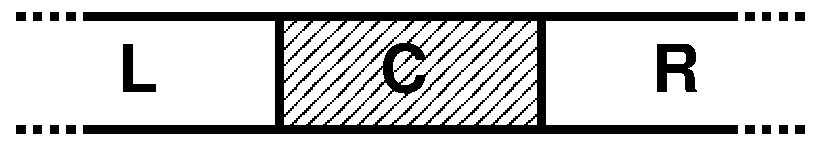
\includegraphics[width=0.45\textwidth]{fig1}
     \caption{A conductor described by the Hamiltonian $H_C$, connected
              to two semi-infinite leads $L$ and $R$, through the coupling
              matrices $h_{LC}$ and $h_{CR}$. \label{fig:LCR} }
   \end{center}
\end{figure}

It is well known that any solid (or surface) can be
viewed as an infinite (semi-infinite in the case of surfaces)
stack of principal layers with nearest-neighbor interactions
\cite{lee-joan81prb,lee-joan81prb1}. This corresponds to
transforming the original system into a linear chain of principal
layers. For a lead-conductor-lead system, the conductor can be
considered as one principal layer sandwiched between two
semi-infinite stacks of principal layers. The next sections
are devoted to the computation of the self-energies using the
principal layers approach.

%%%%%%%%%%%%%%%%%%%%%%%%%%%%%%%%%%%%%%%%%%%%%%%%%%%%%%%%%%%%%%%%%%%

\subsubsection{Transmission through a bulk system.} 
\label{ss:bulk}
%
Within the principal layer approach, the matrix elements
of Eq.~(\ref{eq:GF_def}) between layer orbitals yield a series of
matrix equations for the Green's functions:
%
%
\begin{eqnarray}
\label{serie}
    (\omega -H_{00}) G_{00} & = & I + H_{01}G_{10}\\
\nonumber
    (\omega -H_{00}) G_{10} & = & H_{01}^\dagger G_{00} + H_{01}G_{20}\\
\nonumber
                        \dots\\
\nonumber
    (\omega -H_{00}) G_{n0} & = & H_{01}^\dagger G_{n-1,0} +
                        H_{01}G_{n+1,0}
\end{eqnarray}
%
%
where the finite dimension matrices $H_{nm}$ and
$G_{nm}$ are formed by the matrix elements of the Hamiltonian and
Green's function between the layer orbitals. We assume that in a
bulk system $H_{00}=H_{11}=\dots$ and $H_{01}=H_{12}=\dots$.
Following Refs.~\cite{LopezSancho1,LopezSancho2}, this chain can be
transformed in order to express the Green's function of an
individual layer in terms of the Green's function of the preceding
(or following) one. This is done via the introduction of the
transfer matrices $T$ and $\overline{T}$, defined such that
$G_{10}=TG_{00}$
and $G_{00}=\overline{T}G_{10}$.
Using these definitions, we can write the bulk Green's
function as~\cite{Garcia2}:
%
%
\begin{equation}
    \label{eq:GT} G(\omega) = (\omega - H_{00} - H_{01}T
                  -H_{01}^\dagger \overline{T})^{-1}.
\end{equation}
%
%
The transfer matrix can be easily computed from the
Hamiltonian matrix elements via an iterative procedure, as
outlined in \cite{LopezSancho1,LopezSancho2}. In particular $T$
and $\overline T$ can be written as:
%
%
\begin{eqnarray}
   T &=& t_0 + \tilde{t}_0t_1 + \tilde{t}_0\tilde{t}_1t_2+\ldots+
   \tilde{t}_0\tilde{t}_1\tilde{t}_2\cdots t_n  \, ,\\
\nonumber
   \overline T &=& \tilde{t}_0 + t_0\tilde{t}_1 +t_0t_1\tilde{t}_2
   +\ldots+ t_0t_1t_2\cdots\tilde{t}_n \, ,
\end{eqnarray}
%
%
where $t_i$ and $\tilde{t}_i$ are defined via the recursion
formulas:
%
%
\begin{eqnarray}
   t_i &=& (I -t_{i-1}\tilde{t}_{i-1} - \tilde{t}_{i-1}t_{i-1})^{-1}
   t_{i-1}^2 , \\
   \tilde{t}_i &=& (I -t_{i-1}\tilde{t}_{i-1} -
   \tilde{t}_{i-1}t_{i-1})^{-1} \tilde{t}_{i-1}^2 ,
\nonumber
\end{eqnarray}
%
%
and
%
%
\begin{eqnarray}
   t_0 &=& (\omega - H_{00})^{-1} H_{01}^\dagger,\\
   \tilde{t}_0 &=& (\omega - H_{00})^{-1} H_{01}.
\nonumber
\end{eqnarray}
%
%
\noindent The process is repeated until $t_n,\tilde{t}_n \le
\delta$ with $\delta$ arbitrarily small. Usually, no more than 5 or
6 iterations are required to converge the above sum.

If we compare Eq.~(\ref{eq:GT}) with Eq.~(\ref{gconduct}), 
in the hypothesis of leads and conductors being
of the same material (bulk conductivity), we can identify one
principal layer of the bulk system with the conductor $C$, so that
$H_{00}\equiv H_C$. In particular, by comparing with
Eq.(\ref{gconduct}), we obtain the expression of the self-energies
of the conductor-leads system:
%
%
\begin{equation}
\Sigma_L = H_{01}^\dagger \overline T, \;\;\;\;\; \Sigma_R = H_{01} T.
\label{eq:sigmabulk}
\end{equation}
%
%
The coupling functions are then obtained~\cite{buon99prb} from the sole
knowledge of the transfer matrices and the coupling Hamiltonian
matrix elements: $\Gamma_L=-{\rm Im}(H_{01}^\dagger \overline T)$ and
$\Gamma_R=-{\rm Im}(H_{01} \overline T)$.

%%%%%%%%%%%%%%%%%%%%%%%%%%%%%%%%%%%%%%%%%%%%%%%%%%%%%%%%%%%%%%%%%%%%

\subsubsection{Transmission through a left lead-conductor-right lead
(LCR) system.} \label{ss:LCR}
%
The procedure outlined above can also be applied to the
case of electron transmission through one or more interfaces,
between different media. For the calculation of conductances in
realistic experimental geometry, the method can be expanded to the
general configuration of a Left-lead-Conductor-Right-lead (LCR)
systems --- as displayed in Fig~.\ref{fig:LCR}. To study this case
we make use of the Surface Green's Function Matching (SGFM)
theory, pioneered by~\cite{Garcia1,Garcia2}.

We have to compute the Green's function $G_I$, where the
subscript $I$ refers to the interface region composed of two
principal layers --- one in each media --- (L, C, R in our case).
Using the SGFM method, $G_I$ is calculated from the bulk Green's
function of the isolated systems,  and the coupling between the
two principal layers at the two sides of the interface. Via the
calculation of the transmitted and reflected amplitudes of an
elementary excitation that propagates from one medium to another,
it can be shown that the interface Green's function obeys the
following secular equation~\cite{Garcia2}:
%
%
\begin{eqnarray}
\nonumber G_{LCR}&=& \left(
\begin{array}{ccc}
G_{L} & G_{LC} & G_{LR}\\
G_{CL} & G_{C} & G_{CR}\\
G_{RL} & G_{RC} & G_{R}\\
\end{array}
\right) \\ &=& \left(
\begin{array}{ccc}
\omega -H^L_{00} - (H^L_{01})^\dagger \overline T & -H_{LC} & 0\\
-H_{CL} & \omega -H_{C} & -H_{CR}\\
0 & -H_{RC} & \omega -H^R_{00} - H^R_{01} T \\
\end{array}
\right)^{-1}. \label{secular1}
\end{eqnarray}
%
%
where $H_{nm}^{\{L,R\}}$ are the block matrices of the
Hamiltonian between the layer orbitals in the left and right leads
respectively, and $T_{\{L,R\}}$ and $\overline{T}_{\{L,R\}}$ are
the appropriate transfer matrices. The latter are easily computed
from the Hamiltonian matrix elements via the iterative procedure
already described in the bulk case (Sec.\ref{ss:bulk}).
Correspondingly, $H_{LC}$ and $H_{CR}$ are the coupling matrices
between the conductor and the leads principal layers in contact
with the conductor.
It is straightforward to obtain in the form of
Eq.(\ref{gconduct}), $G_C = (\omega -H_C -\Sigma_L
-\Sigma_R)^{-1}$, where $\Sigma_{L}$ and $\Sigma_R$ are the
self-energy terms due to the semi-infinite leads, and
identify~\cite{buon99prb}:
%
%
\begin{equation}
  \begin{array}{ccl}
  \Sigma_L(\omega) & = & H_{LC}^\dagger \, (\omega -H_{00}^L-(H_{01}^L)^\dagger
                   \overline T_L)^{-1} \, H_{LC},\\ 
  \Sigma_R(\omega) & = & H_{CR} \, (\omega
                  -H_{00}^R-H_{01}^R T_R)^{-1} \, H_{CR}^\dagger.
  \end{array}
\end{equation}
%
%
The transmission function in the LCR geometry can then
be derived from Eq.(\ref{eq:T}) and (\ref{eq:gamma}).
%
The knowledge of the conductor's Green's function $G_C$
gives also direct information on the electronic spectrum of the
system via the spectral density of states:
%
%
\begin{equation}
   N(\omega)= -\frac{1}{\pi} {\rm Im}[{\rm Tr}(G_C(\omega))].
\end{equation}
%
%
We have assumed a truly one-dimensional chain of
principal layers, which is physical only for systems like
nanotubes or quantum wires that have a definite
quasi-one-dimensional character. The extension to a truly
three-dimensional case is straightforward using Bloch functions in
the directions perpendicular to the transport axis. The introduction
of the principal layer concept implies that along the direction of
the layer expansion the system is described by an infinite set of
$k_\bot$ while $k_\|$ are still good quantum numbers for the
problem. The above procedure effectively reduces the
three-dimensional system to a set of non-interacting
linear-chains, one for each $k_\|$~\cite{lee-joan81prb,lee-joan81prb1}. 
We can then use the usual $k$-point summation techniques to evaluate the
quantum conductance: 
%
%
\begin{equation}
    T(\omega) = \sum_{k_\|} w_{k_\|}T_{k_\|}(\omega)
\end{equation}
%
%
where $w_{k_\|}$ are the relative weights of the different $k_\|$
in the irreducible wedge of the surface Brillouin 
zone~\cite{Baldereschi:1}.

%%%%%%%%%%%%%%%%%%%%%%%%%%%%%%%%%%%%%%%%%%%%%%%%%%%%%%%%%%%%%%%%%%%


\subsection {Maximally localized Wannier functions}\label{subsec:wannier}
%
\subsubsection{Definition of the problem}
%
Bloch orbitals cannot be used directly to evaluate
electronic transport with the method outlined in Sec.~\ref{subsec:tran}. 
As we have pointed out, quantum conductance
is computed starting from the knowledge of the lattice Green's
function, whose calculation relies on a localized orbital
representation. Bloch
orbitals, that are intrinsically delocalized, have to be
transformed into {\em localized} functions in order to construct
the sparse, short-ranged matrix elements of the Hamiltonian. The
core of our proposed methodology is to use m{\em
aximally-localized Wannier functions} (WFs) for the system
considered. These are the most natural choice for a set of
localized orbitals that still span the same Hilbert space of the
Hamiltonian eigenfunctions: they allow to bridge plane-wave
electronic structure and lattice Green's function calculations in
a coherent fashion.

A Wannier function $w_{n{\bf R}}({\bf r})$, labeled by
the Bravais lattice vector {\bf R}, is usually defined via a
unitary transformation of the Bloch functions $\psi_{n{\bf
k}}({\bf r})$ of the $n$th band:
%
%
\begin{equation}
w_{n{\bf R}}({\bf r})=\frac{V}{(2\pi)^3}\int_{BZ}\psi_{n{\bf k}}({\bf r})
e^{-i{\bf k}\cdot{\bf R}} d^3k,
\label{wf}
\end{equation}
%
%
where V is the volume of the unit cell and the
integration is performed over the entire Brillouin Zone. It is
easy to show that the WFs defined as above form an orthonormal
basis set, and that any two of them, for a given index $n$ and
different ${\bf R}$ and ${\bf R^\prime}$, are just translational
images of each other. Note that, as WFs are
(continuous) linear combinations of Bloch functions with different
energies, they do not represent stationary states, but still span
the original Hilbert space.

The {\em ab-initio} eigenstates are well-defined,
modulus an arbitrary ${\bf k}$-dependent phase factor; thus, the
definition above does not lead to a unique set of Wannier
functions~\cite{kohn,kohn1}, since the electronic structure
problem is invariant for the transformation $\psi_{n{\bf k}}
\rightarrow e^{\phi_n({\bf k})} \psi_{n{\bf k}} $. Besides this
freedom in the choice of phases $\phi_n({\bf k})$ for the Bloch
functions, there is a more comprehensive gauge freedom stemming
from the fact that the many-body wavefunction is actually a Slater
determinant: a unitary transformation between orbitals will not
change the manifold, and will not change the total energy and the
charge density of the system. In all generality, starting with a
set of ${\mathcal N}$ Bloch functions with periodic parts
$u_{n{\bf k}}$, we can constructs infinite sets of ${\mathcal N}$
WFs displaying different spatial characteristics:
%
%
\begin{equation}
    w_{n{\bf R}}({\bf r})=\frac{V}{(2\pi)^3}\int_{BZ}
    \left[ \sum_m U_{mn}^{({\bf k})}
    \psi_{m{\bf k}}({\bf r}) \right]
    e^{-i{\bf k}\cdot{\bf R}} d^3k.
    \label{eq:MLWF}
\end{equation}
%
%
The unitary matrices $U^{({\bf k})}$ include also the
gauge freedom on phase factors afore mentioned~\cite{nicola}. \\

\noindent The present \WANT\ method is based on a localization algorithm
that allows to transform a set of Bloch functions -- calculated by means
of {\it ab initio} approaches -- into a unique set of Maximally localized
Wannier functions, as proposed by Marzari and Vanderbilt
in 1997~\cite{nicola}. The formulation of this minimum-spread
criterion extends the concept of \emph{localized molecular
orbitals}, proposed by Boys~\cite{boys} for molecules, to the
solid-state case. However, its generality allows to deal with both
``extended'' (periodic and disordered) systems as well as with
``isolated'' clusters and molecules, in the limit of large
supercells.

\subsubsection{Localization procedure}
%
For our purposes, we need to transform the Bloch
eigenstates in WFs with the narrowest spatial
distribution. Following the procedure proposed by Marzari and
Vanderbilt~\cite{nicola}, we search the particular unitary
matrix $U_{mn}^{({\bf k})}$ that transform the Bloch eigenstates
in the WFs with the narrowest spatial distribution.

A measure of the spatial delocalization of WFs is given
by a {\em Spread Operator} $\Omega$, defined as the sum of the
second moments of all the Wannier functions in a reference cell:
%
%
\begin{equation}
    \Omega=\sum_n [\langle r^2 \rangle_n - \langle {\bf r}
    \rangle_n^2] , \label{omega}
\end{equation}
%
%
where the sum is over a selected  group of bands, and
%
%
\begin{eqnarray}
    \langle {\bf r} \rangle_n &=&\langle {\bf 0}n | {\bf r} | {\bf 0}n \rangle, \\
    \nonumber
    \langle r^2 \rangle_n &=& \langle {\bf 0}n | r^2 | {\bf 0}n \rangle .
    \label{position}
\end{eqnarray}
%
%
The value of the spread $\Omega$ depends on the choice
of unitary matrices $U^{({\bf k})}$; thus  it is possible to
evolve any arbitrary set of $U^{({\bf k})}$ until we reach the stationarity
condition:
%
%
\begin{equation}
   \frac {\delta \Omega_{\bf k}}{\delta U^{({\bf k})}}=0
   \label{minimo}
\end{equation}
%
%
At the minimum, we obtain the matrices
$U^{({\bf k}), ML}$ that transform the first-principles
$\psi_{n{\bf k}}^{FP}({\bf r})$ into the {\em maximally-localized
WFs}, according to Eq.~(\ref{eq:MLWF}).
If we restrict to the case of {\bf k}-point mesh
calculations, we can use finite differences in reciprocal space to
evaluate the derivatives of Eq.~(\ref{minimo}). For this purpose we
rewrite the expectation values $\langle \mathbf{r} \rangle$ and 
$\langle r^2 \rangle $ as proposed by Blount~\cite{blount}:
%
%
\begin{eqnarray}
\label{eq:pos_k}
\langle {\bf 0}n | {\bf r} | {\bf 0}n  \rangle &=& i \frac{1}{N}
\sum_{ {\bf k} } e^{ +i{\bf k}\cdot{\bf R} } \langle u_{ {\bf k}n
}| \nabla_{\bf k} | u_{ {\bf k}n },  \rangle\\
%
\nonumber
\langle {\bf 0}n | r^2 | {\bf 0}n \rangle\ &=& \frac{1}{N} \sum_{
{\bf k}} e^{+i{\bf k}\cdot{\bf R}} \langle u_{ {\bf k}n }|
\nabla^2_{\bf k} | u_{ {\bf k}n }  \rangle, 
\end{eqnarray}
%
%
where $| u_{ n{\bf k} }  \rangle = e^{-i{\bf k}\cdot{\bf
r}} | \psi_{ n{\bf k} }  \rangle$ is the periodic part of the Bloch
function. Making the assumption that the BZ has been discretized
into a uniform {\bf k}-point mesh, and letting $ \mathbf{b} $ being 
the vectors
that connect a mesh point to its near neighbors, we can define the
overlap matrix between Bloch orbitals as:
%
%
\begin{equation}
   \label{overlap}
   M^{ ( \mathbf{k},\mathbf{b}) }_{ mn } = \langle u_{ m\mathbf{k} }| 
        u_{ n\mathbf{k}+\mathbf{b} }  \rangle = 
        \langle \psi_{ m \mathbf{k} } | e^{-i\mathbf{k}\mathbf{b}} | 
        \psi_{ n \mathbf{k}+\mathbf{b}} \rangle .
\end{equation}
%
%
Using the expression of the gradient  in terms of finite
differences and substituting $M^{ ({\bf k}, {\bf b})}_{ mn }$ in
Eq.~(\ref{eq:pos_k}) we obtain the expressions for $\langle \mathbf{r} \rangle$
and $\langle r^2 \rangle $
to be used in the localization procedure:
%
%
\begin{eqnarray}
\label{position2}
   \langle \mathbf{r} \rangle_{n} &=& -\frac{1}{N}
          \sum_{ \mathbf{k},\mathbf{b} } 
           w_b \, \mathbf{b} \, \text{Im} 
          \, \text{Ln} M^{ ({\bf k}, {\bf b})}_{ nn } \\ \nonumber
   \langle r^2 \rangle_n &=&  \frac{1}{N} \sum_{ {\bf k,b} } w_b
   \left[ \left( 1- |M^{ ({\bf k}, {\bf b}}_{ nn }|^2 \right) +
          \left( \text{Im}\, \text{Ln} M^{ ({\bf k}, {\bf b})}_{ nn } \right)^2 
   \right]
\end{eqnarray}
%
%
Here, $w_b$ are the weights of the $\mathbf{b}$-vectors, and
must satisfy the completeness condition $\sum_{\mathbf{b}} w_b
b_{\alpha}b_{\beta}= \delta_{{\alpha}{\beta}}$. Substituting the
above expression into Eq.~(\ref{omega}), we obtain the expression
for the spread operator as a function of the overlap matrix $M^{
({\bf k}, {\bf b})}_{ mn }$.

In order to calculate the gradient in Eq.~(\ref{minimo}),
we consider the first order change in $\Omega$ arising from an
infinitesimal transformation $U_{mn}^{({\bf k})} = \delta_{mn} +
dW_{mn}^{({\bf k})}$, where $dW$ is an infinitesimal antiunitary
matrix ($dW^{\dag} = - dW$). The gauge transformation rotates the
wave functions according to Eq.~(\ref{eq:MLWF}) into $| u_{ {\bf k}n }
\rangle \to | u_{ {\bf k}n } \rangle + \sum_mdW_{mn}^{({\bf k})}|
u_{ {\bf k}m } \rangle $. Following the elegant description of
Ref. \cite{nicola}, we obtain the final expression for the
gradient of the spread functional:
%
%
\begin{equation}
   \label{grad_fin}
   G^{({\bf k})}=\frac{\delta \Omega}{dW^{({\bf k})}}= 4 \sum_{ {\bf
   b} } w_b \left( \frac {R^{{\bf k,b})} -R^{({\bf
   k,b}) \, \dagger}}{2} - \frac {T^{({\bf k,b})}+T^{({\bf
   k,b}) \, \dagger}}{2i} \right)  
\end{equation}
%
%
where
%
%
\begin{equation}
   R_{mn}^{ ({\bf k,b}) } = M_{mn}^{ ({\bf k,b}) } M_{nn}^{ ({\bf
   k,b})\ast} ;\qquad T_{mn}^{ ({\bf k,b}) }= \frac{ M_{mn}^{ ({\bf
   k,b}) } } { M_{nn}^{ ({\bf k,b}) } } \left[ \text{Im}\, \text{Ln} M_{nn}^{({\bf
   k,b})} + {\bf b}\cdot \langle {\bf r} \rangle_n \right].
\end{equation}
%
%
Note that the entire expression $G^{({\bf k})}$ is a
function of the overlap matrices $M^{ ({\bf k,b}) }$.  The
minimization of the spread functional $\Omega$ is obtained via
steepest descent or conjugate gradient schemes.
The procedure does not require the updating of wavefunctions, but only
of the overlap and unitary matrixes. This is the most demanding task 
(scaling as $N^3$) for each iteration in Wannier localization.

Wannier functions obtained with the above procedure
should be almost real, except for an overall phase factor. 
This conjecture can also be used as a check of the convergence of the
localization procedure.
It is important to
notice that whenever a Born-von Karman discretization of the
Brillouin Zone is introduced, even the above-mentioned WFs are not
truly localized, but will be periodic in real-space, with a {\em
superperiodicity} determined by the BZ discretization. The truly
isolated limit is recovered only in the case of continuous BZ
integrations. This is easily seen remembering that $ \psi_{n{\bf
k}}({\bf r})= u_{n{\bf k}}({\bf r}) e^{i{\bf k}\cdot{\bf r}} $,
and $� u_{n{\bf k}}({\bf r}) $ has the periodicity of the direct
lattice; thus the phase factors $ e^{i{\bf k}\cdot{\bf r}}� $
determine the {\em superperiodicity} of the $ \psi_{n{\bf k}} $
themselves.

In the standard language of electronic-structure
calculations, if the $ \psi_{n{\bf k}} $ have ${\bf k}$'s that are
restricted to a uniform Monkhorst-Pack mesh, they will all be
periodic with a wavelength inversely proportional to the spacing
of the mesh; this periodicity is consequently inherited by the
WFs. For $\mathcal N$ {\bf k}-points along a direction of the BZ,
the WFs will repeat along the corresponding direction every
$\mathcal N$ cells. A dense mesh of {\bf k}-points guarantees that
the adjacent replicas of a WF are sufficiently far and do not
interact. However, even the case of $\Gamma$-sampling is
encompassed by the above formulation. In this case the neighboring
{\bf k}-points for $\Gamma$ are given by the homologous
$\Gamma$-points of the neighboring cells. In this case the algebra
becomes simpler and an equivalent real-space formulation is
preferred \cite{Silvestrelli,gammaUS}.

The method described above works properly in the case of
{\em isolated groups} of bands. A Bloch band is called {\em
isolated} if it does not become degenerate with any other band
anywhere in the BZ. Conversely, a group of bands is said to form a
{\em composite group} if bands are inter-connected by degeneracy,
but are {\em isolated} from all the other bands~\cite{nicola}. On
the other hand to study quantum conductance in extended systems we
often need to compute WFs for a subset of energy bands that are
entangled or mixed with other bands. Most often we are interested
in the states that lie in the vicinity of the Fermi level of a
conductor in a restricted energy range. Since the unitary
transformations $U^{({\bf k})}$ mix energy bands at each {\bf
k}-point, any arbitrary choice of states inside a prescribed
window will affect the localization properties of WFs unless
energy gaps effectively separate the manifold of interest from
higher and lower bands.
%
This problem has been solved by Souza, Marzari, and
Vanderbilt~\cite{ivo2}, introducing an additional disentanglement
procedure that automatically extracts the best
possible manifold of a given dimension from the states falling in
a predefined energy window. This is the generalization to {\em
entangled} or metallic cases of the maximally-localized WF
formulation. The procedure relies on minimizing the subspace
dispersion across the Brillouin Zone, and effectively extracts the
bands of interest from the overall band structure.

In practice, first we select a desired number of bands
in an energy window; then we determine the optimally-connected
subspace that can be extracted from that band structure; and
finally proceed with a standard localization procedure inside
the selected subspace. 
The resulting orbitals have the same good localization properties, and
allow to apply our formalism to arbitrary systems, independently
of the insulating or metallic nature of the band manifold. It
should be stressed that the WFs obtained in the later case are not
the WFs of the occupied subspace (that would exhibit poor
localization properties), but are those of a well connected,
continuous subspace that in general will contain both occupied and
unoccupied Bloch functions.

%%%%%%%%%%%%%%%%%%%%%%%%%%%%%%%%%%%%%%%%%%%%%%%%%%%%%
\subsubsection{Conditioned localization and penalty functionals}
\label{subsubsec:penalty}
The above described formalism adopts a localization criterion which is 
somehow {\it global}: the functional we want to minimize is the total spread, 
while we are often interested in the localization of 
each Wannier function in the selected set.
In this scenario it may happen that, in order to gain 
localization in the total spread one or more WFs may move their centers out of the
system ({\it e.g.} in the vacuum) and therefore make the remaining functions 
lleave to better localize. In this cases the final WF set is useless from our point of
view.

We therefore introduce the idea of {\it conditioned} localization adding some 
further {\it penalty} functional to the total spread. 
These penalty functionals may be use to drive the Wannier localization towards the
achievement of some required feature.
It maybe interesting {\it e.g.} to fix the problem of WFs moving in the vacuum region
to add a {\it spring} potential driving the functions to have their centers 
as close as possible to the positions we like. The form of the penalty functional 
is therefore:
%
%
\begin{equation}
\label{eq:penalty}
   \Omega_P = A \, \sum_{n} \, w_n\, \left[ \, \langle \mathbf{r} \rangle_n 
                            - \mathbf{r}_{n0} \, \right]^2 ,
\end{equation}
%
%
where $A$ is the functional amplitude, $w_n$ a weight, and $\mathbf{r}_{n0}$ 
is the chosen target position for the $n-$th WF. 
After some tedious algebra it is possible to write and explicit form for the 
derivative of this functional wrt $U^{(\mathbf{k})}$. This is then used to compute
the penalty contribution to the gradient during the minimization of the functional.
Setting to zero some weights $w_n$ we are also able to selectively switch off the 
conditioning on some WFs. 
Obviously many different kinds of such penalty functionals may be written.
We note that this procedure does not alter physical quantities such as the 
polarization, which is infact independent of the particular unitary rotations chosen
for the localization. 
The conditioned minimization fo Eq.~(\ref{eq:penalty}) is implemented in \WANT; 
see Sec.~\ref{sec:input} for more details about how to setup the input file.

%%%%%%%%%%%%%%%%%%%%%%%%%%%%%%%%%%%%%%%%%%%%%%%%%%%%%
\subsubsection{Real space hamiltonians}
%
In order to calculate the conductance according to the
prescriptions outlined in Sec.~\ref{subsec:tran}, we need as an input
the matrix elements of the Hamiltonian calculated on a localized
basis: in our case, it is the minimal basis of the
maximally-localized WFs. 
Assuming a BZ
sampling fine enough to eliminate the interaction with the
WF periodic images, we can simply compute the WF Hamiltonians 
$H_{ij}(\mathbf{R}) = \langle w_{i{\bf 0}} | H | w_{j{\bf R}} \rangle$,
from the unitary rotations $U^{({\bf k})}$ obtained in the localization
procedure.

In the Bloch representation we have by definition 
$H_{mn}(\mathbf{k}) = \epsilon_{m\mathbf{k}} \delta_{m,n}$.
Moving to the Wannier basis we have: 
%
%
\begin{equation}
H^{(rot)}({\bf k})=U^{({\bf k}) \, \dagger} \, H ({\bf
k})\, U^{({\bf k})}.
\label{rot}
\end{equation}
%
%
Next we Fourier transform $H^{(rot)}({\bf k})$ into the
corresponding set of Bravais lattice vectors $\{ \mathbf{R} \}$:
%
%
\begin{equation}
    H_{ij}({\bf R})=\frac{1}{N_{kp}} \sum_{\bf k}
    e^{-i{\bf k}\cdot {\bf R}} \, H^{(rot)}_{ij}({\bf k}) 
\label{hrrot}
\end{equation}
%
%




% Installation
\newpage
%%%%%%%%%%%%%%%%%%%%%%%%%%%%%%%%%%%%%%%%%%%%%%%%%%%%%%%%%%
%  Copyright (C) 2005 WanT group                         %
%  This file is distributed under the terms of the       %
%  GNU General Public License.                           %
%  See the file `License'  in the root directory of      %
%  the present distribution,                             %
%  or http://www.gnu.org/copyleft/gpl.txt                %
%%%%%%%%%%%%%%%%%%%%%%%%%%%%%%%%%%%%%%%%%%%%%%%%%%%%%%%%%%

\thispagestyle{empty}
\section{Installation procedure}\label{section:install}

\noindent \underline {NOTES}: (i) The present version of the code
adopts the installation procedure of PWSFC (for more details see
also www.pwscf.org). (ii) This installation procedure is still
experimental, and only a limited number of architectures are
currently supported.
Installation procedure is also reported in the {\bf docs/README.install} file.\\

\noindent Installation is a two-step procedure:
\begin{enumerate}
\item ``cd'' to the top directory of the \WANT\ tree (that should be
the one where this file is), and issue this command at the shell
prompt:\\
$./$configure
\item Now run:\\
     make target\\
\end{enumerate}
\noindent where ``target'' is one (or more) of the following:
disentangle, wannier, conductor, bands, blc2wan, plot. Running
"make" without arguments prints a list of available targets.\\

\noindent Cross-compilation is not currently supported.

%----------------------------------------------------------------------
%First step : configuring
%----------------------------------------------------------------------

\subsection{Step one: configuring} ``configure'' is a GNU-style configuration script,
automatically generated by GNU Autoconf.  (If you want to play
with it, its source file is ``conf/configure.ac''; you may also
want to edit ``conf/make.sys.in'')  It generates the following
files:
\begin{displaymath}
\begin{array}{ll}
  \textrm{\$TOPDIR/make.sys}        &      \textrm{compilation settings and flags}\\
  \textrm{\$TOPDIR/*/makedeps.sh}   &      \textrm{dependencies, per
  source directory}
\end{array}
\end{displaymath}
\noindent where \$TOPDIR is the top directory of the \WANT\ source
tree.\\

\noindent ``.dependencies'' files are actually generated by the
``makedeps.sh'' shell script.  If you modify the program sources,
you might have to rerun it.  Note that you must run it from the
directory it is in.\\

\noindent To force using a particular compiler, or compilation
flags, or libraries, you may set the appropriate environment
variables when running the configuration script.  For example:

\begin{description}
  \item ./configure CC=gcc CFLAGS=-O3 LIBS=``-llapack -lblas
  -lfftw''
\end{description}

\noindent Some of those environment variables are:
\begin{displaymath}
\begin{array}{ll}
  \textrm{TOPDIR}       &\textrm{: top directory of the \WANT\ tree (defaults to `pwd`)}\\
  \textrm{F90, F77, CC} &\textrm{: Fortran 90, Fortran 77, and C compilers}\\
  \textrm{CPP}          &\textrm{: source file preprocessor (defaults to "\$CC -E")}\\
  \textrm{LD}           &\textrm{: linker (defaults to \$F90)}\\
  \textrm{CFLAGS, FFLAGS,}  &\textrm{ }\\
  \textrm{F90FLAGS, CPPFLAGS, LDFLAGS} &\textrm{: compilation flags}\\
  \textrm{LIBDIRS}      &\textrm{: extra directories to search for libraries (see below)}\\
\end{array}
\end{displaymath}

\noindent You should always be able to compile the \WANT\ suite of
programs without having to edit any of the generated files.  If
you ever have to, that should be considered a bug in the
configuration script and you are encouraged to submit a bug
report.\\

\noindent \underline {IMPORTANT}: \WANT\ can take advantage of
several
optimized numerical libraries:\\
\noindent - ESSL on AIX systems (shipped by IBM)\\
\noindent - MKL together with Intel compilers (shipped by Intel,
free for non-commercial use)\\
\noindent  - ATLAS (freely downloadable from
http://math-atlas.sourceforge.net/)\\
\noindent  - FFTW (freely downloadable from
http://www.fftw.org/)\\

\noindent The configuration script attempts to find those
libraries, but may fail if they have been installed in
non-standard locations. You should look at the LIBS environment
variable (either in the output of the configuration script, or in
the generated ``make.sys'') to check whether all available
libraries were found.\\

\noindent If any libraries weren't found, you can rerun the
configuration script and pass it a list of directories to search,
by setting the environment variable LIBDIRS; directories in the
list must be
separated by spaces.  For example:\\

\begin{description}
  \item ./configure LIBDIRS=``/opt/intel/mkl/mkl61/lib/32
  /usr/local/lib/fftw-2.1.5''
\end{description}

\noindent If this still fails, you may set the environment
variable LIBS manually and retry.  For example:\\

\begin{description}
  \item ./configure LIBS=``-L/cineca/prod/intel/lib -lfftw -llapack
  -lblas''
\end{description}

\noindent Beware that in this case, you must specify *all* the
libraries that you want to link to.  The configuration script will
blindly accept the specified value, and will *not* search for any
extra libraries.\\

\noindent If you want to use the FFTW library, the ``fftw.h"
include file is also required.  If the configuration script wasn't
able to find it, you can specify the correct directory in the
INCLUDEFFTW environment variable. For example:\

\begin{description}
  \item ./configure INCLUDEFFTW=``/cineca/lib/fftw-2.1.3/fftw''
\end{description}

%----------------------------------------------------------------------
%Second step : compiling
%----------------------------------------------------------------------
\subsection{Step two: compiling}
\noindent Here is a list of available compilation targets:
\begin{displaymath}
\begin{array}{llll}
  \textrm{make all}        &  \textrm{compile} & \textrm{wannier/disentangle.x} &\textrm{(step 1)}\\
  \textrm{}                &  \textrm{}       & \textrm{wannier/wannier.x}     &\textrm{(step 2)}\\
  \textrm{}                &  \textrm{}       & \textrm{wannier/bands.x}       &\textrm{(post proc)}\\
  \textrm{}                &  \textrm{}       & \textrm{wannier/plot.x}        &\textrm{(post proc)}\\
  \textrm{}                &  \textrm{}       & \textrm{wannier/blc2wan.x}     &\textrm{(post proc)}\\
  \textrm{}                &  \textrm{}       & \textrm{transport/conductor.x} &\textrm{(step 3)}\\
  \textrm{make clean}      &  \textrm{remove}  & \textrm{Object files and
  executables}&  \textrm{}\\
    \textrm{make veryclean}      &  \textrm{remove}  & \textrm{Configuration files too}&  \textrm{}
\end{array}
\end{displaymath}

\noindent \underline {IMPORTANT}: If you change any compilation or
precompilation options after a previous (successful or failed)
compilation, you must run ``make clean'' before recompiling,
unless you know exactly which routines are affected by the changed
options and how to force their recompilation.

\subsection{List of directories}
Within the top directory of the \WANT\ tree there are the
following directories:

\newdimen\descindent \descindent = 8pc
{\noindent \leftskip = \descindent \parskip = .5\baselineskip
\llap{\hbox to \descindent{\bf conf\hfil}}%
includes the configuration and compilation files\par

\noindent\llap{\hbox to \descindent{\bf docs\hfil}}%
includes the documentation files and manuals \par

\noindent\llap{\hbox to \descindent{\bf iotk\hfil}}%
includes the files for the iotk input/output interface \par

\noindent\llap{\hbox to \descindent{\bf transport\hfil}}%
includes the source files and modules of for program conductor.x
\par

\noindent\llap{\hbox to \descindent{\bf wannier\hfil}}%
includes the source files and modules of for programs
disentangle.x, wannier.x, bands.x, plot.x, blc2wan.x \par

\noindent\llap{\hbox to \descindent{\bf bin\hfil}}%
includes links of all the executable file *.x \par

\noindent\llap{\hbox to \descindent{\bf include\hfil}}%
includes the environmental file *.h \par

\noindent\llap{\hbox to \descindent{\bf libs\hfil}}%
includes source file for internal libraries \par

\noindent\llap{\hbox to \descindent{\bf tests\hfil}}%
includes tutorial examples for the use of \WANT\ suite of
codes\par

\noindent\llap{\hbox to \descindent{\bf utility\hfil}}%
includes some useful tools for \WANT\ use. \par}


% Input and output files
\newpage
%%%%%%%%%%%%%%%%%%%%%%%%%%%%%%%%%%%%%%%%%%%%%%%%%%%%%%%%%%
%  Copyright (C) 2005 WanT group                         %
%  This file is distributed under the terms of the       %
%  GNU General Public License.                           %
%  See the file `License'  in the root directory of      %
%  the present distribution,                             %
%  or http://www.gnu.org/copyleft/gpl.txt                %
%%%%%%%%%%%%%%%%%%%%%%%%%%%%%%%%%%%%%%%%%%%%%%%%%%%%%%%%%%

\thispagestyle{empty}
\section{How to run \WANT\ : a step by step description}\label{section:run}

\noindent \underline {NOTE}: At present the \WANT\ code is
implemented to work as post processing of DFT 
calculations done using the \PWSCF package (\PWSCFURL); we
will refer to that code in the following.\\

\noindent Following the theoretical description of
Section~\ref{section:intro}, the evaluation of transport
properties requires three separate steps:

\begin{enumerate}
\item Calculation of DFT electronic structure
\item Calculation of maximally-localized Wannier functions
\item Calculation of quantum conductance
\end{enumerate}

\noindent \underline{IMPORTANT}: For a correct results, the
following steps \textbf{MUST} be done in the reported order.

\subsection{Preliminary Steps: DFT
Calculations}\label{subsection:run_dft}
\renewcommand{\theenumi}{\roman{enumi}}
\renewcommand{\labelenumi}{\theenumi)}
\begin{enumerate}
%
\item Self-consistent calculation using the \PWSCF code.\\
      \noindent For the description of the input and for further details see the \PWSCF
      manual.
      %
\item Bandstucture calculation.\\
      \noindent  Starting from the self-consistent charge
      calculated in point $(1)$, we calculate the Bloch functions for a
      {\bf REGULAR {\bf k}-point grid in the COMPLETE Brillouin Zone}; Gamma point
      must be included. Reduction of \textbf{k}-points due to time-reversal 
      symmetry is not (yet) allowed. The complete list of 
      \textbf{k}-points should be specified in the {\tt K\_POINTS} card. 
      The simple program
      {\tt kgrid.f90} in {\tt \$TOPDIR/utility }can be used to generate non-symmetrized 
      Monkhorst-Pack grids.
      %
\item From \PWSCF to the Wannier code.\\
      \noindent Use the post processing
      {\tt pw\_export.x} (distributed in the \PWSCF package 
      %
      \footnote{The export utility is already distributed in the 
      Qantum-Espresso v3.0, but a patch to include it also in versions v2.1.x is
      available at \WANTURL{} or \PWSCFURL{}. When using v.3.0.0 do not compile with
      the {\tt -D\_\_NEWPUNCH} pre-processor flag.} 
      ),
      %
      to extract the input data necessary for the following Wannier
      calculations
      from \PWSCF output datafile. Data will be stored in the
      newly-created directory {\tt \$prefix.export/}.
\end{enumerate}

\noindent \underline{NOTE}: Steeps (i-iii) should be be run, using the
parallel version of the code, paying attention to use the same
number of processors. From this point to the end, instead, the
code is scalar.

%%%%%%%%%%%%%%%%%%%%%%%%%%%%%%%%%%%%%%%%%%%%%%%%%%%%%%%%%%%%%%
\subsection {Calculation of maximally-localized Wannier
functions}\label{subsection:run_wannier}

Following the list of input parameters as in
Section~\ref{sec:input} (also reported in the {\tt README.input} file
in {\tt \$TOPDIR/docs/}) and the examples in directory {\tt \$TOPDIR/tests/}, 
create your own input file, that will be used for the following two steps (a-b).
\renewcommand{\theenumi}{\alph{enumi}}
\renewcommand{\labelenumi}{\theenumi)}
%
%
\begin{enumerate}
\item {\tt disentangle.x}: Starting from the data stored at level (iii), 
      the code selects the working energy window. From there
      it will extract a selected number ($N$) of WFs to setup the 
      Hilbert subspace for Wannier localization.
      For each \textbf{k}-point, the energy window {\bf must}
      contain a number of bands not lower than $N$.
      It is possible to use an inner window (inside the working one) to
      treat frozen-states, for details see Ref.~\cite{ivo2}:
      these frozen Bloch-states will be kept as they are in the Wannier subspace.
      % 
      Trial Wannier centers are not mandatory in this step (depending
      on the {\tt subspace\_init} flag).
      The code produces a standard output with the main results,
      and two internal files: {\tt \$prefix\_\$postfix.ovp} and
      {\tt \$prefix\_\$postfix.space} . The former keeps trace of the 
      computed overlap and projection integrals (to be re-used in further 
      or restarted calculations) while the latter describe the wannier optimal 
      subspace.
      %

\item {\tt wannier.x}: the code reads the same input of {\tt disentangle.x} and
      performs the localization
      procedure leading to the maximally localized WFs. 
      The optimal unitary matrices $U(\mathbf{k})$ governing the transformation between
      Bloch and Wannier states are obtained.
      In this step different trial centers can be used, but it is a standard procedure
      to keep those used in the {\tt disentangle.x} run.
      {\tt wannier.x} produces a standard output with describing the iterative
      path to the optimally localized WFs. 
      The code also writes two internal data-files: {\tt \$prefix\_\$postfix.wan}
      containing the $U(\mathbf{k})$ and {\tt \$prefix\_\$postfix.ham} with the 
      hamiltonian matrix elements on the Wannier basis.
      %
\end{enumerate}
%
%

\noindent
Further physical information may be obtained as external
post-processing of the Wfs calculation. They are not necessary for
the transport calculation, but they may be useful for a
better understanding of the intrinsic electronic properties of the
system. These codes require a separate input, to be generated
following Sec.~\ref{sec:input} or the file
{\tt \$TOPDIR/docs/README.input} .

%
%
\begin{itemize}
%
\item {\tt bands.x}: the code computes the interpolated band-structure
      of the system along selected direction in the Brillouin Zone.
      The comparison with indipendently calculated DFT eigenvalues is
      a nice test to check the localization of the obtained WFs.
      When they are well behaved ({\it i.e.} localized), only few $\mathbf{R}$ lattice 
      vectors are required to described the Hamiltonian on the Wannier basis 
      [$H_{ij}(\mathbf{R})$]
      Starting with a small set of $\mathbf{k}$ in the DFT calculation
      we obtain the Hamiltonian on the related (small) set of lattice vectors. 
      When WFs are well localized 
      the Hamiltonian is fully described on this set of $\mathbf{R}$ and we can
      diagonalize it for an arbitrary large set of $\mathbf{k}$ points 
      (as a post-processing of the Wannier code). This is the
      interpolation of the band structure using WFs. If they are not localized
      we are essentially throuwing away some non-negligible matrix elements 
      in the Hamiltonian representation, and the bands
      are not accurate. Typical unphysical oscillations appears in these cases.
      % 
      The code produces three files {\tt \$prefix\_\$postfix\_dftband.dat,
      \$prefix\_\$postfix\_wanband.dat} and {\tt \$prefix\_\$postfix\_intband.dat}
      which cab be used for a direct visualization.
      %

\item {\tt plot.x}: this is an utility to plot WFs in real space.
      The plotting region can be tuned and a genereic number of WFs can be
      handled in a single run.
      The real or immaginary parts of the WFs as well as their squared moduli are
      allowed fields to be plotted.
      The code produces plot files in various formats (txt, gaussian cube, xsf, plt) 
      allowing the use of standard open source visualization-packages
      such as gOpenMol or xCrysDen. Output files are labelled as 
      {\tt \$prefix\_\$postfix\_WF\$type\_\$num.\$fmt}, where {\tt \$type} can be
      {\tt R, I, M} according to the plotted field (real or immaginary part, squared 
      modulus), {\tt \$num} is the index of the chosen WF and {\tt \$fmt} is the
      output format. If needed, an auxiliary file with the atomic structure 
      in the {\tt xyz} format is also produced.
      %
\item {\tt blc2wan.x}: transforms a generic (eventually dynamic) operator 
      given on the Bloch eigenstates basis $A_{mn}(\mathbf{k}) =
      \langle \psi_{m\mathbf{k}} |\, \widehat{A}(\omega) \,| 
      \psi_{n\mathbf{k}} \rangle$ to the WFs representation. 
      Using the unitary matrices $U(\mathbf{k})$ calculated during the Wannier localization
      (b) and the definition of the Wannier subspace in terms of the Bloch eigenstates
      (a), $\widehat{A}(\omega)$ is described in terms of the matrix elements
      $A_{ij}(\mathbf{R}) = \langle w_{i\mathbf{0}} |\, \widehat{A}(\omega) \,| 
      w_{j\mathbf{R}} \rangle$ .
\end{itemize}

%%%%%%%%%%%%%%%%%%%%%%%%%%%%%%%%%%%%%%%%%%%%%%%%%%%%%%%%%%%%%%%

\subsection {Calculation of electronic transport}
\label{subsection:transport}

Using the hamiltonian matrices calculated in step (b) we can
calculate both the {\em bulk} and the {\em two-terminal} transmittance.
Input file may be generated following Sec.~\ref{sec:input}
or the file {\tt README.input} in {\tt \$TOPDIR/docs}. The main result of the 
calculation is the quantum transmittance across the conductor region
which is written on file {\tt \$SCRATCH/cond.dat}. Conductance is given
in $2e^2/h$ units. Calculations are performed using the Fisher-Lee formula
according to Sec.~\ref{subsec:tran}.
As an auxiliary piece of information, the density of states (DOS) projected on
the conductor is also writte in {\tt \$SCRATCH/dos.dat}.
This DOS is computed as the trace of the conductor Green's function
$ N(E) = -(1/\pi)\, \text{Im} \, \text{Tr}\, G_C(E)$.

Except the special case of the bulk transmittance (see below), the systems one is
interested in are generally not periodic along the transport direction. This does not
in principle avoid a 2D periodicity in the orthogonal plane. The use of 
2D mesh of $\mathbf{k}$-points in this context is implemented in the present 
version of the code.  \\

%%%%%%%%%%%%%%%%%%%%%%%%%%%%%%%%%%%%%%%%%
%
%
\begin{figure}
   \centering
   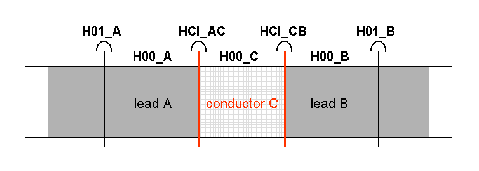
\includegraphics[clip,width=0.6\textwidth]{acb}
   \caption{Schematic definitions for Hamiltonian block matrices used in 
	    transport calculations. \label{fig:matrix_naming}}
\end{figure}
%
%
\noindent 
Before discussing in more ditail the actual calculations performed by
the transport code, we precisely define the adopted convention for the
names of the real-space ({\i.e.} WF) Hamiltonian blocks.  
Given a conductor (C) connected to left (L) and right (R) leads, containing
respectively $N_C$, $N_L$ and $N_R$ WFs, 
we define the following matrices (see Fig.~\ref{fig:matrix_naming}): \\

%
%
\begin{table}[h]
%
\begin{tabular}{lllll}
\texttt{H00\_L} &=& $N_L\times N_L$ on-site hamiltonian
of the leads L & (from L-bulk calc.)\\
\texttt{H01\_L} &=& $N_L\times N_L$ hopping hamiltonian
of the leads L & (from L-bulk calc.) \\
\texttt{H00\_R} &=& $N_R\times N_R$ on site hamiltonian
of the leads R & (from R-bulk calc.) \\
\texttt{H01\_R} &=& $N_R\times N_R$ hopping hamiltonian
of the leads R & (from R-bulk calc.) \\
\texttt{H00\_C} &=& $N_C\times N_C$ on site hamiltonian
of the conductor C & (from C-supercell calc.) \\
\texttt{H\_LC}  &=& $N_L\times N_C$ coupling
between lead L and conductor C & (from C-supercell calc.) \\
\texttt{H\_CR}  &=& $N_C\times N_R$ coupling
between conductor C and lead R & (from C-supercell calc.)
%
%
\end{tabular} \\
%
\caption {Main Hamiltonian blocks neede for transport calculation 
          \label{tab:hamiltonian_blocks} }
\end{table}
%
%
%
\noindent
In the general case we need to compute the electronic structure and
WFs for three different regions L, C, R.
Very often one is interested in a situation where the leads are composed
of the same material. We wil discuss in more detail this case, the being 
treatable in the same way except fo a more complicated geometry in the
conductor region.

First we note that the conductor calculation should contain part of the leads
in the simulation cell, in order to treat the interface from frist principles.
The amount of lead layers to be included should be converged upto the local 
electronic structure of the bulk lead is reached at the edges of the supercell.
This convergence can be controlled taking a look at the 
hamiltonian matrix elements 
on Wannier states located in the lead region
({\it e.g.} nearest neighbour interactions).
Note that this is a physical condition related to the need for a matching of different
calculations and not to the peculiar use of WFs as a basis: nevertheless the smaller
the WFs the more indipendend on the environment are the matrix elements, which leads
to a faster convergence.

As from Tab.~\ref{tab:hamiltonian_blocks}, the {\tt H00\_C} term can be obtained directly
from the conductor supercell calculation. The on-site block ($\mathbf{R}=\mathbf{0}$)
is automatically selected.
The same is true in general for the lead-conductor coupling (consider for instance
{\tt H\_CR}): here the rows of the matrix are related to (all) the WFs in the conductor
reference cell while the columns usually refer to the some 
of them in the nearest neighbor cell along transport direction (say {\it e.g.} the
third lattice vector). The {\tt H\_CR} Hamiltonian we are interested in is therefore a 
$N_C \times N_R$ submatrix of the $\mathbf{R}=(0,0,1)$ block.
In order to understand which rows and columns should enter the submatrix, 
we need to identify some WFs in the conductor with those obtained for bulk lead 
calculation. 
This assumption is strictly correlated with that about the local
electronic structure at the edge of the conductor supercell: the more we reach
the electronics of the leads, the more WFs will be similar to those of bulk leads.
As before, the smaller the WFs, the more indipendent of the environment they are.
In this way we can extract the lead-conductor coupling matrices
directly from the supercell conductor calculation. Much care must be 
taken in this step in order to avoid numerical noise. 
See Sec.~\ref{sec:input} for the input file details.

The missing Hamiltonians ({\tt H00\_x, H01\_x}, where {\tt x=L,R}) can be obtained from
direct calculations for the bulk leads and are taken from the 
$\mathbf{R}=(0,0,0)$ and $\mathbf{R}=(0,0,1)$ blocks respectively 
(as from Tab.~\ref{tab:hamiltonian_blocks}).
All these Hamiltonian matrix elements are related to a zero of the energy scale 
set at the Fermi energy of the computed system 
(the top of valence band for semiconductors). It is not therefore guaranteed the
zero of the enrgy to be exactly the same when moving from the conductor to the leads
(which comes from different calculations. )
In order to
match the hamiltonian matrices at the boundary, it is necessary to
check that the corresponding diagonal elements (the only affected by a shift in the
energy scale) 
of {\tt H00\_L, H00\_C and H00\_R} matrices are aligned 
(see the end of the {\tt wannier.x} output-file to 
easily find these elements). If not, a rigid shift may be applied.

Alternatively, the {\tt H00\_x} and {\tt H01\_x} matrices may be obtained from the 
conductor supercell calculation too.
We need to identify the WFs corresponding to some principal layer of the leads
and extract the corresponding rows and columns. This procedure is not affected by
any energy-offset problem, but larger supercells should be used in order to obtain
environment (conductor) indipendent matrices. See the tests to check the 
numerical performance of these schemes.
%
\\

\noindent The transport code distributed within the \WANT package is 
{\tt conductor.x} which calculates both the 
{\em bulk} and the {\em two-terminal} transmittance for the systems.
While in the former case we 
only need the {\tt H00\_C} and the {\tt H\_CR} matrices, the whole complexity
of input data described above is managed in the latter.



% Input and output files
\newpage
%%%%%%%%%%%%%%%%%%%%%%%%%%%%%%%%%%%%%%%%%%%%%%%%%%%%%%%%%%
%  Copyright (C) 2005 WanT group                         %
%  This file is distributed under the terms of the       %
%  GNU General Public License.                           %
%  See the file `License'  in the root directory of      %
%  the present distribution,                             %
%  or http://www.gnu.org/copyleft/gpl.txt                %
%%%%%%%%%%%%%%%%%%%%%%%%%%%%%%%%%%%%%%%%%%%%%%%%%%%%%%%%%%

\thispagestyle{empty}
\section{How to setup input files}\label{sec:input}

\noindent According to the methodological scheme of Sec.~\ref{sec:run},
it is necessary to use separate input files at
the different step of the \WANT\ procedure.\\

\noindent Input files are organized using several {\tt NAMELIST}s,
followed by other fields with more massive data {\tt CARDS}. Namelists are
begin with the flag {\tt \&NAMELIST } and end with the
"$/$'' bar. The order of variables within a namelist is
arbitrary. Most variables have default values mandatory.
If a variable is not explicitly defined in the input file,
its default value is assumed. Other variables are mandatory and must be
always supplied.
In the following we report the list and the description
of the details of each required input file.

\subsection{Input for DFT-PW calculations}
\noindent {\bf Step 1. i-ii:} {\tt pw.x}
\\
\noindent \WANT\ is currently interfaced with \PWSCF code. For the
description of the input for steps 1-2 (Sec. \ref{sec:run})
and for further details see the \PWSCF manual at \PWSCFURL .\\

\noindent {\bf Step 1. iii:}  {\tt pw\_export.x}
\\
\noindent Input file layout: \\

%
%
\begin{tabular}{c}
  {\tt \&INPUTPP } \\
    ... \\
  $/$
\end{tabular}
%
%
\\

%
%
\begin{centering}
\rule{2.5in}{0.01in} List of variables \rule{2.5in}{0.01in}
\end{centering}\\

\newdimen\descindent \descindent = 8pc
{\noindent \leftskip = \descindent \parskip = .5\baselineskip
\llap{\hbox to \descindent{\tt prefix\hfil}}%
{\sc string} \\ the first part of the name of all the files written by
the code. When using \PWSCF for the DFT calculation, {\tt prefix} should be the
same.\\ {\sc default} = {\tt mandatory} \par

\noindent\llap{\hbox to \descindent{\tt outdir\hfil}}%
{\sc string} \\ the scratch directory where the massive data-files will
be written.\\  {\sc default} = {\tt "./" }\par

\noindent\llap{\hbox to \descindent{\tt pseudo\_dir\hfil}}%
{\sc string} \\directory containing pseudopotential (PP) files.\\
{\sc default} = {\tt "./"} \par

\noindent\llap{\hbox to \descindent{\tt psfile(i)\hfil}}%
{\sc string} \\ files containing $i$-th pseudopotential, where $i=1, N_{\text{type}}$.
PP numbering must follow the ordering defined in the input of {\tt pw.x} . \\
{\sc default} =  {\tt ""} \par
\par

\noindent\llap{\hbox to \descindent{\tt single\_file\hfil}}%
{\sc logical} \\ if {\tt .TRUE.} a single output file is produced, otherwise
  the output is a directory with few files.\\
{\sc default} = {\tt .FALSE. }\par

\noindent\llap{\hbox to \descindent{\tt ascii\hfil}}%
{\sc logical}  \\ if {\tt .TRUE.} output files are textual, otherwise
they are partly binary.\\
{\sc default} = {\tt .FALSE.} \par}\bigskip


%%%%%%%%%%%%%%%%%%%%%%%%%%%%%%%%%%%%%%%%%%%%%%%%%%%%%%%%%%%%
\subsection{Input for Wannier function calculations}
\noindent {\bf Step 2. a-b:} {\tt disentangle.x wannier.x}\\
\noindent Both codes for WF calculation use the same input file.\\

\noindent Input file layout: \\

%
%
\begin{tabular}{l}
{\tt \&CONTROL }\\
   ... \\
  / \\
  \\
{\tt \&SUBSPACE }\\
   ... \\
  $/$ \\
  \\
{\tt \&LOCALIZATION }\\
   ... \\
  $/$ \\
  \\
{\tt  WANNIER\_CENTERS } {\tt ( "crystal" $\mid$ "angstrom" $\mid$ "bohr" $\mid$ "alat") }\\
  $\langle${\tt type}$_1\rangle \qquad    \langle${\tt specific\_fmt}$\rangle$ \\
  ... \\
  $\langle${\tt type}$_N\rangle \qquad    \langle${\tt specific\_fmt}$\rangle$
\end{tabular}
%
%
\\
\\

\begin{centering}
\rule{2.2in}{0.01in} Namelist {\tt \&CONTROL } \rule{2.2in}{0.01in}
\end{centering}\\

\newdimen\descindent \descindent = 8pc
{\noindent \leftskip = \descindent \parskip = .5\baselineskip
\llap{\hbox to \descindent{\tt prefix\hfil}}%
{\sc string} \\ the first part of the name of all the files written by
the code.\\ {\sc default} = {\tt mandatory} \par

\noindent\llap{\hbox to \descindent{\tt postfix\hfil}}%
{\sc string} \\ the tail of the names of the above mentioned files (useful {\it e.g.} to
distinguish among different calculations having a common part).\\
{\sc default} = {\tt ""} \par

\noindent\llap{\hbox to \descindent{\tt work\_dir\hfil}}%
{\sc string} \\ the scratch directory where the massive data-files will be written.\\
{\sc default} = {\tt "$./$" }\par

\noindent\llap{\hbox to \descindent{\tt title\hfil}}%
{\sc string} \\ the title of the calculation.\\
{\sc default} = {\tt "Wannier Transport Calculation"} \par

\noindent\llap{\hbox to \descindent{\tt restart\_mode\hfil}}%
{\sc string} \\ {\tt ( "from\_scratch" $\mid$ "restart" ) }\\
define whether to restart a previous calculation;
at the moment the {\tt "restart"} choice implies to give the value
{\tt "from\_file"} to the input
variables {\tt overlaps, projections,
start\_mode\_dis} and {\tt start\_mode\_wan}
(see below for their meanings).\\ {\sc default} = {\tt "from\_scratch"} \par

\noindent\llap{\hbox to \descindent{\tt verbosity\hfil}}%
{\sc string} \\ {\tt ( "low" $\mid$ "medium" $\mid$ "high" ) }
\\the level of detail of the textual output files.\\
{\sc default} = {\tt "medium"} \par

\noindent\llap{\hbox to \descindent{\tt overlaps\hfil}}%
{\sc string} \\ {\tt ( "from\_scratch" $\mid$ "from\_file" ) }\\
determine how to get overlap integrals:\\
{\tt "from\_scratch"}:  overlaps are calculated from wfs\\
{\tt "from\_file"}:     overlaps are read from a previous data file.
In this second case the dimensions of the problem should be the same as in the
original calculation.\\
{\sc default} = {\tt "from\_scratch"} \par

\noindent\llap{\hbox to \descindent{\tt projections\hfil}}%
{\sc string} \\ {\tt ( "from\_scratch" $\mid$ "from\_file" ) }\\
determine how to get projections integrals:
the meaning of the options is as for {\tt overlaps} variable.\\
{\sc default} = {\tt "from\_scratch"} \par

\noindent\llap{\hbox to \descindent{\tt assume\_ncpp\hfil}}%
{\sc logical} \\ if {\tt .TRUE.} avoids the reading of pseudopotential files
assuming that the DFT calculation has been performed using norm-conserving
pseudopotentials (no knowledge of them is required in the \WANT\ calculation
in this case).\\
{\sc default} = {\tt .FALSE.} \par

\noindent\llap{\hbox to \descindent{\tt unitary\_thr\hfil}}%
{\sc real} \\ threshold for the check of matrix unity.\\
{\sc default} = {\tt 1.0d-6} \par
}\bigskip

\begin{centering}
\rule{2.2in}{0.01in} Namelist {\tt \&SUBSPACE} \rule{2.2in}{0.01in}
\end{centering}\\

\newdimen\descindent \descindent = 8pc
{\noindent \leftskip = \descindent \parskip = .5\baselineskip
\llap{\hbox to \descindent{\tt dimwann\hfil}}%
{\sc integer} \\ the number of Wannier functions, {\it i.e.} the dimension of the
Wannier subspace.
\\ {\sc default} = {\tt mandatory} \par

\noindent\llap{\hbox to \descindent{\tt win\_min\hfil}}%
{\sc real} \\ the lower limit [eV] of the energy window containing the Bloch states
forming the Wannier subspace).\\
{\sc default} = {\tt $-\infty$} \par

\noindent\llap{\hbox to \descindent{\tt win\_max\hfil}}%
{\sc real} \\ the upper limit [eV] of the energy window described above.\\
{\sc default} = {\tt $+\infty$} \par

\noindent\llap{\hbox to \descindent{\tt froz\_min\hfil}}%
{\sc real} \\ the lower limit [eV] of the energy window containing {\it frozen}
Bloch states: they will be taken as they are in the Wannier subspace and do not enter
the disentanglement procedure. \\
{\sc default} = {\tt $-\infty$} \par

\noindent\llap{\hbox to \descindent{\tt froz\_max\hfil}}%
{\sc real} \\ upper limit [eV] of the frozen window described above.\\
{\sc default} = {\tt $-\infty$} \par

\noindent\llap{\hbox to \descindent{\tt alpha\_dis\hfil}}%
{\sc real} \\ mixing parameter for the disentangle iterative procedure.\\
{\sc default} = {\tt 0.5} \par

\noindent\llap{\hbox to \descindent{\tt maxiter\_dis\hfil}}%
{\sc integer} \\  maximum number of iterations during the disentangle procedure.\\
{\sc default} = {\tt 1000} \par

\noindent\llap{\hbox to \descindent{\tt nprint\_dis\hfil}}%
{\sc integer} \\  every {\tt nprint\_dis} iterations in disentangle minimization write to
stdout.\\ {\sc default} = {\tt 10} \par

\noindent\llap{\hbox to \descindent{\tt nsave\_dis\hfil}}%
{\sc integer} \\  every {\tt nsave\_dis} iterations save subspace data to disk.\\
{\sc default} = {\tt 10} \par

\noindent\llap{\hbox to \descindent{\tt use\_blimit\hfil}}%
{\sc logical} \\   if {\tt .TRUE.}, $\mathbf{b}$-vectors are set to zero
when calculating overlap augmentations.
This essentially means we are doing a sort of thermodynamic limit
even if this is not consistent with the actual kpt grid. The {\tt .TRUE.} value
should be considered for debug purposes.\\ {\sc default} = {\tt .FALSE.} \par

\noindent\llap{\hbox to \descindent{\tt disentangle\_thr\hfil}}%
{\sc real} \\  threshold for convergence of the iterative disentangle procedure.\\
{\sc default} = {\tt 1.0d-8} \par

\noindent\llap{\hbox to \descindent{\tt subspace\_init\hfil}}%
{\sc string} \\  {\tt ( "randomized" $\mid$ "lower\_states" $\mid$ "upper\_states" $\mid$ \\
"center\_projections" $\mid$ "from\_file" ) }\\
Determine how the trial subspace is chosen\\
{\tt "randomized"}   : random starting point is chosen\\
{\tt "lower\_states"} : the lower {\tt dimwann} bands from DFT calculation are
                 used to define the subspace\\
{\tt "upper\_states"} : the upper {\tt dimwann} bands from DFT calculation are
                 used to define the subspace\\
{\tt "center\_projections"} : a subspace is extracted from the DFT bands
                 by means of a projections on the given Wannier trial-centers
                 (see the card {\tt WANNIER\_CENTERS})\\
{\tt "from\_file"} : subspace initialization is read from an existing data file;
                 this is the choice used during restart.\\
{\sc default} = {\tt "center\_projections"} \par

\noindent\llap{\hbox to \descindent{\tt spin\_component\hfil}}%
{\sc string} \\  {\tt ( "up" $\mid$ "down" $\mid$ "none")}\\
defines whether the calculation is spin polarized and if the case
which spin component is to be treated.\\
{\sc default} = {\tt "none"} \par
}\bigskip

\begin{centering}
\rule{2.2in}{0.01in} Namelist {\tt \&LOCALIZATION} \rule{2.2in}{0.01in}
\end{centering}\\

\newdimen\descindent \descindent = 8pc
{\noindent \leftskip = \descindent \parskip = .5\baselineskip
\llap{\hbox to \descindent{\tt wannier\_thr\hfil}}%
{\sc real} \\ threshold for convergence of the iterative Wannier minimization.
\\ {\sc default} = {\tt 1.0d-6} \par

\noindent\llap{\hbox to \descindent{\tt alpha0\_wan\hfil}}%
{\sc real} \\ mixing parameter during the steepest-descent minimization steps. \\
{\sc default} = {\tt 0.5} \par

\noindent\llap{\hbox to \descindent{\tt alpha1\_wan\hfil}}%
{\sc real} \\ mixing parameter during the conjugate-gradient minimization steps. \\
{\sc default} = {\tt 0.5} \par

\noindent\llap{\hbox to \descindent{\tt maxiter0\_wan\hfil}}%
{\sc integer} \\ maximum number of steps for the steepest descent
minimization (first part).\\ {\sc default} = {\tt 500} \par

\noindent\llap{\hbox to \descindent{\tt maxiter1\_wan\hfil}}%
{\sc integer} \\ maximum number of steps for the conjugate-gradient minimization
(second part).\\ {\sc default} = {\tt 500 }\par

\noindent\llap{\hbox to \descindent{\tt nprint\_wan\hfil}}%
{\sc integer} \\ every {\tt nprint\_wan} iterations in wannier minimization write to stdout.\\
{\sc default} = {\tt 10 }\par

\noindent\llap{\hbox to \descindent{\tt nsave\_wan\hfil}}%
{\sc integer} \\ every {\tt nsave\_wan} iterations save subspace data to disk.\\
{\sc default} = {\tt 10 }\par

\noindent\llap{\hbox to \descindent{\tt ncg\hfil}}%
{\sc integer} \\ every {\tt ncg} iterations in the second minimization part,
do a steepest-descent step.\\ {\sc default} = {\tt 3 }\par

\noindent\llap{\hbox to \descindent{\tt localization\_init\hfil}}%
{\sc $\quad$ string} \\
{\tt ( "no\_guess" $\mid$ "randomized" $\mid$ "center\_projections"
$\mid$ "from\_file" )}\\
 Determine how the Wannier localization is started\\
{\tt "no\_guess"} : disentangle states are used as starting point
                 without any further localization guess\\
{\tt "randomized"} : a random rotation is applied to the states found by
                 the disentangle procedure\\
{\tt "center\_projections"} : a subspace is extracted from the DFT bands
                 by means of a projections on the given Wannier trial-centers \\
{\tt "from\_file"} : subspace initialization is read from an existing data file;
                 this is the choice used during restart. \\
{\sc default} = {\tt "center\_projections"} \par

\noindent\llap{\hbox to \descindent{\tt ordering\_mode\hfil}}%
{\sc string} \\ {\tt ( "none" $\mid$ "spatial" $\mid$ "spread" $\mid$ "complete" ) } \\
specifies whether to order the computed Wannier functions and
              which ordering criterion adopt\\
{\tt "none"}:      no ordering is performed\\
{\tt "spatial"}:   ordering based on WF center positions\\
{\tt "spread"}:    ordering based on WF increasing spreads\\
{\tt "complete"}:  {\tt spatial} + {\tt spread}. \\
{\sc default} = {\tt "none" }\par

\noindent\llap{\hbox to \descindent{\tt a\_condmin\hfil}}%
{\sc real} \\ the amplitude of the conditioned minimization functional. If set to zero
              ordinary minimization is performed.\\
{\sc default} = {\tt 0.0} \par

\noindent\llap{\hbox to \descindent{\tt niter\_condmin\hfil}}%
{\sc integer} \\ the number of steps for which minimization is conditioned.\\
{\sc default} = $\begin{array}{ll}
           {\tt maxiter0\_wan + maxiter1\_wan}     & \textrm{(if {\tt a\_condmin}} \neq 0.0)\\
           {\tt 0}                                 & \textrm{(otherwise)}
           \end{array}$ \par

\noindent\llap{\hbox to \descindent{\tt dump\_condmin\hfil}}%
{\sc real} \\ the dumping factor for {\tt a\_condmin} during the conditioned minimization.
              If the dumping factor is specified, after {\tt niter\_condmin}
              iterations {\tt a\_condmin}
              is dumped according to {\tt a\_condmin = a\_condmin $*$ dump\_condmin}
              at each iteration.\\
{\sc default} = {\tt 0.0} \par
}
\bigskip

\begin{centering}
\rule{2.0in}{0.01in} Card {\tt WANNIER\_CENTERS} \rule{2.0in}{0.01in}
\end{centering}\\

\noindent {\tt WANNIER\_CENTERS}
{\tt ( "crystal" $\mid$ "angstrom" $\mid$ "bohr" $\mid$ "alat") }\\

\noindent Aside the tag {\tt WANNIER\_CENTERS}, units for positions maybe specified:\\
%
%
\begin{tabular}{ll}
\texttt{"crystal"}  & : relative coordinates on the basis of $\mathbf{a}_1,\mathbf{a}_2,\mathbf{a}_3$
                                direct lattice vector (default)\\
\texttt{"bohr"}     & : cartesian coordinates in Bohr\\
\texttt{"alat"}     & : cartesian coordinates in units of the
                        first lattice vector module\\
\texttt{"angstrom"} & : cartesian coordinates in Angstrom
\end{tabular}
%
%
\\

\noindent Next the card contains {\tt dimwann} lines giving the trial centers for the WFs.
Depending on the $\langle${\tt type}$\rangle$ flag at the beginning of the line,
formats are different.\\

\noindent $\langle${\tt type}$\rangle$ may assume the values: {\tt "atomic" , "1gauss", "2gauss" }\\
%
%
\begin{displaymath}
\begin{array}{lllllll}
\texttt{if ( type == "atomic" )}  & \rightarrow
& \texttt{atomic}
&\quad \texttt{iatomic}
&\quad \texttt{l} \quad  \texttt{m}
&\quad \texttt{ }
&\quad \texttt{[weight]}\\
\texttt{if ( type == "1gauss" )}  & \rightarrow
& \texttt{1gauss}
&\quad \texttt{x} \quad  \texttt{y} \quad  \texttt{z}
&\quad \texttt{l} \quad  \texttt{m}
&\quad \texttt{rloc}
&\quad \texttt{[weight]} \\
\texttt{if ( type == "2gauss" )}  & \rightarrow
& \texttt{2gauss}
&\quad \texttt{x} \quad  \texttt{y} \quad  \texttt{z}
&\quad \texttt{xx} \quad  \texttt{yy} \quad  \texttt{zz}
&\quad \texttt{rloc}
&\quad \texttt{[weight]}
\end{array}
\end{displaymath}
%
%
\bigskip

\noindent {\tt type == "1gauss}"\\
\noindent The trial center is given by a single gaussian set at a given position with a given
angular momentum. Standard positions are usually atomic sites or bond midpoints.\\

\newdimen\descindent \descindent = 8pc
{\noindent \leftskip = \descindent \parskip = .5\baselineskip
\llap{\hbox to \descindent{\tt x, y, z\hfil}}%
{\sc real} \\ define the position of the trial function. Units maybe specified aside
            the tag {\tt WANNIER\_CENTERS}, see above for more details. \par

\noindent\llap{\hbox to \descindent{\tt l, m\hfil}}%
{\sc integer} \\ are the angular momentum quantum numbers for the spherical harmonics
giving the angular part of the trial center. {\tt l} can be set equal to 0, 1, or 2,
(and {\tt m} values are then as usual) for standard spherical harmonics or {\tt l} == -1
indicating the sp3 geometry. Here spherical harmonics are the real ones:\\

%
%
$\begin{array}{lllll}
\texttt{l == -1:}   &\texttt{m = -4}  &\rightarrow   & \texttt{ 1,1,-1}              &\texttt{dir}\\
\texttt{}           &\texttt{m = -3}  &\rightarrow   & \texttt{ 1,-1, 1}             &\texttt{dir}\\
\texttt{}           &\texttt{m = -2}  &\rightarrow   & \texttt{-1, 1,1}              &\texttt{dir}\\
\texttt{}           &\texttt{m = -1}  &\rightarrow   & \texttt{-1,-1,-1}             &\texttt{dir}\\
\texttt{}           &\texttt{m =  1}  &\rightarrow   & \texttt{ 1,1, 1}              &\texttt{dir}\\
\texttt{}           &\texttt{m =  2}  &\rightarrow   & \texttt{ 1,-1,-1}             &\texttt{dir}\\
\texttt{}           &\texttt{m =  3}  &\rightarrow   & \texttt{-1,1,-1}              &\texttt{dir}\\
\texttt{}           &\texttt{m =  4}  &\rightarrow   & \texttt{-1,-1, 1}             &\texttt{dir}\\
\texttt{l == 0:}    &\texttt{m =  0}  &\rightarrow   & \texttt{spherical}            &\texttt{}\\
\texttt{l == 1:}    &\texttt{m = -1}  &\rightarrow   & \texttt{x}                    &\texttt{}\\
\texttt{}           &\texttt{m =  0}  &\rightarrow   & \texttt{z}                    &\texttt{}\\
\texttt{}           &\texttt{m =  1}  &\rightarrow   & \texttt{y}                    &\texttt{}\\
\texttt{l == 2:}    &\texttt{m = -2}  &\rightarrow   & \texttt{x}^2 - \texttt{ y}^2  &\texttt{}\\
\texttt{}           &\texttt{m = -1}  &\rightarrow   & \texttt{xz}                   &\texttt{}\\
\texttt{}           &\texttt{m =  0}  &\rightarrow   & \texttt{3z}^2 - \texttt{ r}^2 &\texttt{}\\
\texttt{}           &\texttt{m =  1}  &\rightarrow   & \texttt{yz}                   &\texttt{}\\
\texttt{}           &\texttt{m =  2}  &\rightarrow   & \texttt{xy}                   &\texttt{}\\
\end{array}$ \par

\noindent\llap{\hbox to \descindent{\tt rloc\hfil}}%
{\sc real} \\ specifies the spread of the gaussian used for the radial part of the
trial WF. Units are Bohr for both {\tt"bohr"} and {\tt"crystal"} and Angstrom for {\tt "angstrom"}
specifier.\par

\noindent\llap{\hbox to \descindent{\tt weight\hfil}}%
{\sc real} \\ this value is required when conditioned minimization is performed. In case,
            it should be set in the interval [0, 1]. It weights the relative importance of
            each center in the penalty functional. Weight = 0 is used to switch off the
            constrain for a given center.\par
}
\bigskip

\noindent {\tt type == "2gauss}"\\
\noindent The trial function is given as the difference between s-symmetry gaussians placed
at the positions selected by the user. This is useful to mimic some antibonding state.\\

\newdimen\descindent \descindent = 8pc
{\noindent \leftskip = \descindent \parskip = .5\baselineskip
\llap{\hbox to \descindent{\tt x, y, z\hfil}}%
{\sc real} \\ as before for {\tt type == "1gauss"}. \par

\noindent\llap{\hbox to \descindent{\tt xx, yy, zz\hfil}}%
{\sc real} \\ as before for {\tt x,y,z} but specify the center of the second gaussian
            used to set up the trial center.  \par

\noindent\llap{\hbox to \descindent{\tt rloc\hfil}}%
{\sc real} \\  as before for {\tt type == "1gauss"}. \par

\noindent\llap{\hbox to \descindent{\tt weight\hfil}}%
{\sc real} \\  as before for {\tt type == "1gauss"}. \par
}
\bigskip

\noindent {\tt type == "atomic}"\\
\noindent Atomic (pseudo)-orbitals from pseudopotential data-files are used as trial functions.
They are specified by the atomic index and the required angular momentum quantum-numbers.\\

\newdimen\descindent \descindent = 8pc
{\noindent \leftskip = \descindent \parskip = .5\baselineskip
\llap{\hbox to \descindent{\tt iatom\hfil}}%
{\sc integer} \\ the index of the chosen atom (ordering is directly taken from DFT data). \par

\noindent\llap{\hbox to \descindent{\tt l, m\hfil}}%
{\sc real} \\ as before for {\tt type == "1gauss"}.\par

\noindent\llap{\hbox to \descindent{\tt weight\hfil}}%
{\sc real} \\ as before for {\tt type == "1gauss"}.\par
}


%%%%%%%%%%%%%%%%%%%%%%%%%%%%%%%%%%%%%%%%%%%%%%%%%%%%%%%%%%%%%%%%%%%%%%%
\subsection{Input for electronic transport calculations}
\noindent {\bf Step 3 : conductor.x}\\
\noindent Both bulk and two-terminal calculations use similar input.
Labels follow the scheme of Sec.~\ref{sec:run}.\\

\noindent Input file layout: \\

%
%
\begin{tabular}{l}
{\tt \&INPUT\_CONDUCTOR }\\
   ... \\
  / \\
  \\
{\tt <HAMILTONIAN\_DATA>} \\
  $\quad$ {\tt <ham$_1$   attr="" />} \\
  $\quad$ ...  \\
  $\quad$ {\tt <ham$_N$   attr="" />} \\
{\tt </HAMILTONIAN\_DATA>}
%
\end{tabular}
%
%
\\

\begin{centering}
\rule{2.2in}{0.01in} Namelist {\tt \&INPUT\_CONDUCTOR} \rule{2.2in}{0.01in}
\end{centering}\\

\newdimen\descindent \descindent = 8pc
{\noindent \leftskip = \descindent \parskip = .5\baselineskip
\llap{\hbox to \descindent{\tt dimL\hfil}}%
{\sc integer} \\ number of sites in the L-lead.
\\ {\sc default} = {\tt 0} \par

\noindent\llap{\hbox to \descindent{\tt dimR\hfil}}%
{\sc integer} \\ number of sites in the R-lead. \\
{\sc default} = {\tt 0} \par

\noindent\llap{\hbox to \descindent{\tt dimC\hfil}}%
{\sc integer} \\ number of sites in the conductor region. \\
{\sc default} = {\tt mandatory} \par

\noindent\llap{\hbox to \descindent{\tt calculation\_type\hfil}}%
{\sc string} \\ {\tt ( "conductor" $\mid$ "bulk" ) }
            determines the kind of calculation to be performed:\\
            {\tt "conductor"}:  ordinary transport calculation for a
                    leads$\mid$conductor$\mid$lead junction\\
            {\tt "bulk"}: transport in a bulk system.\\
            {\sc default}: {\tt "conductor"} \par

\noindent\llap{\hbox to \descindent{\tt transport\_dir\hfil}}%
{\sc integer} \\ transport direction according to crystal axis indexing. \\
{\sc default} = {\tt mandatory} \par

\noindent\llap{\hbox to \descindent{\tt conduct\_formula\hfil}}%
{\sc string} \\ {\tt ( "landauer" $\mid$ "generalized" ) }
            {\tt "landauer"}:  transport is computed using the standard Landauer formula \\
            {\tt "generalized"}: a generalized Landauer formula accounting for a
                 specific correlation correction is used. This case is experiemntal, see
                 Ref.~\cite{ferr+05prl, ferr+05prb} for more details. \\
            {\sc default}: {\tt "landauer"} \par

\noindent\llap{\hbox to \descindent{\tt ne\hfil}}%
{\sc integer} \\ dimension of the energy grid for transmittance and spectral function
            calculation.\\
{\sc default} = {\tt 1000}\par

\noindent\llap{\hbox to \descindent{\tt emin\hfil}}%
{\sc real} \\ lower limit [eV] of the energy grid. \\
{\sc default} = {\tt -10.0} \par

\noindent\llap{\hbox to \descindent{\tt emax\hfil}}%
{\sc real} \\ upper limit [eV] of the energy grid. \\
{\sc default} = {\tt +10.0} \par

\noindent\llap{\hbox to \descindent{\tt delta\hfil}}%
{\sc real} \\ small imaginary part used to get off the real axis in the calculation
            of Green's functions. \\
{\sc default} = {\tt 1.0e-5} \par

\noindent\llap{\hbox to \descindent{\tt nprint\hfil}}%
{\sc integer} \\ every {\tt nprint} energy step write to stdout .\\
{\sc default} = {\tt 20} \par

\noindent\llap{\hbox to \descindent{\tt niterx\hfil}}%
{\sc integer} \\ maximum number of iterations in the calculation of transfer
                 matrices. \\
{\sc default} = { \tt 200} \par

\noindent\llap{\hbox to \descindent{\tt use\_overlap\hfil}}%
{\sc logical} \\ If {\tt .TRUE.} reads the overlap matrices from file,
otherwise basis orthonormality
            is assumed (which is by definition the case of Wannier functions). \\
            {\sc default} : {\tt .FALSE.} \par

\noindent\llap{\hbox to \descindent{\tt use\_correlation\hfil}}%
{\sc logical} \\ If {\tt .TRUE.} correlation corrections are read from file and included
            in the calculation. See also the {\tt datafile\_sgm} variable. \\
            {\sc default} : {\tt .FALSE.} \par

\noindent\llap{\hbox to \descindent{\tt datafile\_C \hfil}}%
{\sc string} \\ Name of the file containing the Wannier Hamiltonian blocks for the
            conductor region. \\
            {\sc default}: {\tt "mandatory"} \par

\noindent\llap{\hbox to \descindent{\tt datafile\_L \hfil}}%
{\sc string} \\ Name of the file containing the Wannier Hamiltonian blocks for the
            L-lead. It is nor required for {\tt bulk} calculations. \\
            {\sc default}: {\tt "mandatory"} if not {\tt calculation\_type == "bulk"} \par

\noindent\llap{\hbox to \descindent{\tt datafile\_R \hfil}}%
{\sc string} \\ as for {\tt datafile\_L} but for R-lead. \\
            {\sc default}: {\tt "mandatory"} if not {\tt calculation\_type == "bulk"} \par

\noindent\llap{\hbox to \descindent{\tt datafile\_sgm \hfil}}%
{\sc string} \\ Name of the file containing the correlation self-energy. It is required only
            when correlation is included in the calculation. \\
            {\sc default}: {\tt "mandatory"} if {\tt use\_correlation == .TRUE.} \par
}
\bigskip

\begin{centering}
\rule{2.0in}{0.01in} Card {\tt <HAMILTONIAN\_DATA>} \rule{2.0in}{0.01in}
\end{centering}\\

\noindent The card {\tt <HAMILTONIAN\_DATA>} is mandatory and specifies
the details about hamiltonian blocks to be used in transport calculation.
It includes a variable number of subtags (XML format)
to be used the order shown below. The name and the number of these subcards
depend on the {\tt calculation\_type} variable:

%
%
\begin{displaymath}
\begin{array}{lll}
\texttt{if ( calculation\_type = "bulk" )}         & \rightarrow &
                                                     \textrm{two subcards are needed}\\
\texttt{}                                          & \texttt{}   &
                                                     \texttt{<H00\_C>},\texttt{<H\_CR>}\\
\texttt{}                                          & \texttt{}   & \textbf{}\\
\texttt{if ( calculation\_type = "conductor" )}    & \rightarrow &
                                                     \textrm{seven subcards are needed}\\

\texttt{}                                          & \texttt{}   &
                                                     \texttt{<H00\_C>},
                                                     \texttt{<H\_CR>},\texttt{<H\_LC>},\\
\texttt{}                                          & \texttt{}   &
                                                     \texttt{<H00\_L>},\texttt{<H01\_L>},\\
\texttt{}                                          & \texttt{}   &
                                                     \texttt{<H00\_R>}, \texttt{<H01\_R>}\\
\end{array}
\end{displaymath}
%
%

\noindent Names of the subcards refer to Fig.~\ref{fig:matrix_naming} in
Sec.~\ref{subsec:tran}.
Each subcard (tag) may contain a number of attribute, according to the
format (XML compliant):
%
%
\begin{description}
\item
   {\tt <H$_{\text{whatever}}$  cols=""  rows=""  />}
\end{description}
%
%


\newdimen\descindent \descindent = 8pc
{\noindent \leftskip = \descindent \parskip = .5\baselineskip
\llap{\hbox to \descindent{\tt cols (rows) \hfil}}%
{\sc string} \\
the string describing which index should be considered to define the
columns (rows) of the specific {\tt H} submatrix.
The format in the string is quite standard, according {\it e.g.} to the default
for printing programs: \\
{\tt  "1-3,5,7-9" } stands for {\tt "1,2,3,5,7,8,9"}, and so on.
The string {\tt "ALL"} is allowed as well, being equivalent to
{\tt "1-N$_{\text{max}}$"}. \\
{\sc default} = {\tt "ALL"} \par

}
%%%%%%%%%%%%%%%%%%%%%%%%%%%%%%%%%%%%%%%%%%%%%%%%%%%%%%%%%%%%%%%%%%%

\subsection{Input for post-processing calculations}
\subsubsection{bands.x}
\noindent Input file layout: \\

%
%
\begin{tabular}{l}
 {\tt \&INPUT} \\
   ... \\
   / \\
  \\
 {\tt label$\_1$ $\quad$ $k_1$ $k_2$ $k_3$ } \\
  ... \\
 {\tt label$\_N$ $\quad$ $k_1$ $k_2$ $k_3$ } \\
\end{tabular}
%
%
\\

\begin{centering}
\rule{2.2in}{0.01in} Namelist {\tt \&INPUT} \rule{2.2in}{0.01in}
\end{centering}\\

\newdimen\descindent \descindent = 8pc
{\noindent \leftskip = \descindent \parskip = .5\baselineskip
\llap{\hbox to \descindent{\tt prefix\hfil}}%
{\sc string} \\ the first part of the name of all the files written by the code;
              it should be equal to the value given in the main calculations.\\
{\sc default} = {\tt mandatory} \par

\noindent\llap{\hbox to \descindent{\tt postfix\hfil}}%
{\sc string} \\ the tail of the names of the above mentioned files (useful
    {\it e.g.} to distinguish among different calculations having a common part);
    it should be equal to the value given in the main calculations.\\
    {\sc default} = {\tt ""} \par

\noindent\llap{\hbox to \descindent{\tt work\_dir\hfil}}%
{\sc string} \\ the scratch directory where the massive data files will be written.\\
              {\sc default} = {\tt "./"} \par

\noindent\llap{\hbox to \descindent{\tt verbosity\hfil}}%
{\sc string} \\ {\tt ( "low" $\mid$ "medium" $\mid$ "high" ) }\\
              the level of detail of the textual output file.\\
              {\sc default} =  {\tt "medium"} \par

\noindent\llap{\hbox to \descindent{\tt nkpts\_in\hfil}}%
{\sc integer} \\ number of edge $\mathbf{k}$-points defining the directions
on which bands will be calculated.\\
{\sc default}: {\tt mandatory} \par

\noindent\llap{\hbox to \descindent{\tt nkpts\_max\hfil}}%
{\sc integer} \\ maximum number of interpolated $\mathbf{k}$-points. The actual number
of points is calculated in the run and is written in the output file.\\
{\sc default} = {\tt 100} \par

\noindent\llap{\hbox to \descindent{\tt spin\_component\hfil}}%
{\sc string} \\  {\tt ( "up" $\mid$ "down" $\mid$ "none" ) }\\
              define whether the calculation is spin polarized and, if the case,
              which spin component is treated.\\
{\sc default} = {\tt "none"} \par
}\bigskip

\noindent After the {\tt \&INPUT} namelist, a description line for each of the
{\tt nspts\_in} points must be provided. The format is as follows:\\

\noindent $\qquad$ \texttt{label} $\quad$ {\tt $k_1$ $k_2$ $k_3$ } \\

\newdimen\descindent \descindent = 8pc
{\noindent \leftskip = \descindent \parskip = .5\baselineskip
\llap{\hbox to \descindent{\tt label\hfil}}%
{\sc string} \\ a string with the conventional name of the $\mathbf{k}$-point. \par

\noindent\llap{\hbox to \descindent{\tt $k_1$ $k_2$ $k_3$\hfil}}%
{\sc real} \\ components of the $\mathbf{k}$-point vector in units of crystal reciprocal
              lattice \\
              ( {\it i.e.} $ \mathbf{k} = k_1 * \mathbf{b}_1 + k_2 * \mathbf{b}_2 +
              k_3 * \mathbf{b}_3 $). \par
}\bigskip

\subsubsection{plot.x}
\noindent Input file layout: \\

%
%
\begin{tabular}{l}
  {\tt \&INPUT } \\
  ... \\
  / \\
\end{tabular}
%
%
\\

\begin{centering}
\rule{2.2in}{0.01in} Namelist {\tt \&INPUT} \rule{2.2in}{0.01in}
\end{centering}\\

\newdimen\descindent \descindent = 8pc
{\noindent \leftskip = \descindent \parskip = .5\baselineskip
\llap{\hbox to \descindent{\tt prefix\hfil}}%
{\sc string} \\ the first part of the name of all the file written by the code;
              it should be equal to the value given in the main calculations.\\
              {\sc default} = {\tt mandatory} \par

\noindent\llap{\hbox to \descindent{\tt postfix\hfil}}%
{\sc string} \\ the tail of the names of the above mentioned files.
              It should be equal to the value given in the main calculations.\\
              {\sc default} = {\tt ""} \par

\noindent\llap{\hbox to \descindent{\tt work\_dir\hfil}}%
{\sc string} \\ the scratch directory where the massive data files will be written.\\
              {\sc default} = {\tt "./"} \par

\noindent\llap{\hbox to \descindent{\tt wann\hfil}}%
{\sc string} \\ specifies the indexes of the Wannier functions to be plotted.
              It is a string of format {\it e.g.} {\tt "1-3,5,7-9"}
              (analogous to the fmt used to specify pages to standard print utilities)\\
              {\sc default} = {\tt mandatory} \par

\noindent\llap{\hbox to \descindent{\tt datatype\hfil}}%
{\sc string} \\ {\tt ("modulus" $\mid$ "real" $\mid$ "imaginary") }\\
              specifies the type of data plotted:\\
                {\tt "modulus"}:    plot the real space square modulus of the WFs. \\
                {\tt "real"}:       plot the real part (in real space) of the WFs. \\
                {\tt "imaginary"}:  plot the imaginary part (in real space) of the WFs
                              this choice should be intended as a check because WFs
                              are expected to be more or less {\it real}.\\
              {\sc default} = {\tt "modulus"} \par

\noindent\llap{\hbox to \descindent{\tt output\_fmt\hfil}}%
{\sc string} \\ {\tt ( "plt" $\mid$ "txt" $\mid$ "cube" $\mid$ "xsf" ) }\\
              Define the format of the output files to be plotted.
              {\tt "plt"} (read by {\sc gOpenMol}) is binary and smaller than
              {\tt "cube"}, {\tt "xsf"} (read by {\sc xcrysden}) and
              {\tt "txt"}. While {\tt "cube"} and {\tt "xsf"} deal also
              with non-orthorombic lattices, {\tt "txt"} is suitable to be converted
              to further format.\\
              {\sc default} = {\tt "plt"} \par

\noindent\llap{\hbox to \descindent{\tt r1min, r1max\hfil}}%
{\sc real} \\ the starting and ending points of the plotting cell along the
              first direct lattice vector $\mathbf{a}_1$.
              Units of $\mathbf{a}_1$.\\
              {\sc default} = {\tt -0.5, 0.5} \par

\noindent\llap{\hbox to \descindent{\tt r2min, r2max\hfil}}%
{\sc real} \\ as before but for $\mathbf{a}_2$ direction.\\
              {\sc default} = {\tt -0.5, 0.5} \par

\noindent\llap{\hbox to \descindent{\tt r3min, r3max\hfil}}%
{\sc real} \\ as before but for $\mathbf{a}_2$ direction.\\
              {\sc default} = {\tt -0.5, 0.5} \par

\noindent\llap{\hbox to \descindent{\tt assume\_ncpp\hfil}}%
{\sc logical} \\ if using norm-conserving pseudopototentials which are not readable
               by \WANT\ set this value to .TRUE. in order to avoid their reading.\\
              {\sc default} = {\tt .FALSE.} \par

\noindent\llap{\hbox to \descindent{\tt locate\_wf\hfil}}%
{\sc logical} \\ if {\tt .TRUE.} moves the WFs in a unit cell centered around the
    midpoint of the plotting cell. Useful to plot purposes.\\
              {\sc default} = {\tt .TRUE.} \par

\noindent\llap{\hbox to \descindent{\tt spin\_component\hfil}}%
{\sc string} \\ {\tt ( "up" $\mid$ "down" $\mid$ "none" ) }\\
              define whether the calculation is spin polarized and, if the case,
              which spin component is treated.\\
              {\sc default} = {\tt "none"} \par
}\bigskip

\subsubsection{blc2wan.x}
\noindent Input file layout: \\

%
%
\begin{tabular}{l}
  {\tt \&INPUT } \\
  ... \\
  / \\
\end{tabular}
%
%
\\

\begin{centering}
\rule{2.2in}{0.01in} Namelist {\tt \&INPUT} \rule{2.2in}{0.01in}
\end{centering}\\

\newdimen\descindent \descindent = 8pc
{\noindent \leftskip = \descindent \parskip = .5\baselineskip
\llap{\hbox to \descindent{\tt prefix\hfil}}%
{\sc string} \\ the first part of the name of all the file written by the code;
              it should be equal to the value given in the main calculations.\\
              {\sc default} = {\tt mandatory} \par

\noindent\llap{\hbox to \descindent{\tt postfix\hfil}}%
{\sc string} \\ the tail of the names of the above mentioned files.
              It should be equal to the value given in the main calculations.\\
              {\sc default} = {\tt ""} \par

\noindent\llap{\hbox to \descindent{\tt work\_dir\hfil}}%
{\sc string} \\ the scratch directory where the massive data files will be written.\\
              {\sc default} = {\tt "./"} \par

\noindent\llap{\hbox to \descindent{\tt filein\hfil}}%
{\sc string} \\ the name of the file containing the input operator in the Bloch
                representation.\\
              {\sc default} = {\tt mandatory} \par

\noindent\llap{\hbox to \descindent{\tt fileout\hfil}}%
{\sc string} \\ the name of the file containing the computed operator on the
                Wannier basis.\\
              {\sc default} = {\tt mandatory} \par

\noindent\llap{\hbox to \descindent{\tt ascii\hfil}}%
{\sc logical} \\ if {\tt .TRUE.} the output file is written in textual XML format.\\
              {\sc default} = {\tt .FALSE.} \par
}


% trouble shootting
\newpage
%%%%%%%%%%%%%%%%%%%%%%%%%%%%%%%%%%%%%%%%%%%%%%%%%%%%%%%%%%
%  Copyright (C) 2005 WanT group                         %
%  This file is distributed under the terms of the       %
%  GNU General Public License.                           %
%  See the file `License'  in the root directory of      %
%  the present distribution,                             %
%  or http://www.gnu.org/copyleft/gpl.txt                %
%%%%%%%%%%%%%%%%%%%%%%%%%%%%%%%%%%%%%%%%%%%%%%%%%%%%%%%%%%

\thispagestyle{empty}
\section{What to do when things go wrong?}
\label{sec:troubleshoot}
%
This section is not intended to be complete. Here we report
a summary of the most frequent and well-known problems in the
day-by-day practice with \WANT, and some tentative suggestions to
solve them. Please, report any better solution or explanation you
find to the maintainer of this manual to make it more detailed.

%%%%%%%%%%%%%%%%%%%%%%%%%%%%%%%%%%%%%%%%%%%
\subsection{When do things go really wrong ?}
First it is necessary to understand which behaviors should be considered buggy and
which may be conversely related to some failures of the implemented algorithms.
This section is devoted to guide the user to understand whether the code is
properly running or not. \\
%
%
\begin{itemize}
\item   {\bf Stops and crashes.} \\
        When the code stops, it is expected either to have reached the end
        of the calculation (which is marked in the output file by a summary
        of the timing) or to print
        out an error message and to give a fortran stop. Any different behavior
        should be considered a bug and should be reported
        (obviously it may be related to machine dependent problems,
        independently of \WANT).

\item   {\bf Problems connected to memory usage.} \\
        Since the code is still serial, no distribution of the memory among
        CPUs is performed and crashes may result. In these cases, both an
        error message during allocations or a more drastic error (even segmentation
        fault) may occur. The largest amount of memory is used by
        {\tt disentangle.x} (which manage wave-functions), while {\tt wannier.x}
        does not require that much. Post-processing ({\tt bands.x, blc2wan.x})
        do not have special requirement too, while {\tt plot.x} needs a sensible
        amount of memory, about half of {\tt disentangle.x}.

\item   {\bf Convergence in disentanglement minimization.} \\
        The iterative procedure in {\tt disentangle.x} is quite robust.
        Non-monotonic behaviors of the invariant spread are unexpected
        and are probably related to algorithm failures. Although, convergence
        may be very slow, especially when some parameters are not properly set
        (too many empty states in the main energy window, strange numbers of
        requested WFs...) .

\item   {\bf Convergence in Wannier localization.} \\
        In the case of {\tt wannier.x}, convergence is less straightforward.
        Particularly for large systems, it may happen that the total spread first 
        decreases for several iterations and then it suddenly jumps to a much higher
        value.  This cycle may be repeated several times.
        From the expressions for the spread funcitonal in Ref.~\cite{nicola}, we see that
        many evaluations of the imaginary part of complex logarithms are needed. 
        These are the phases of the arguments, which in the present case are the overlap
        integrals. Since logarithm in the complex plane
        is a multivalued function, sudden jumps in the total spread (towards larger
        values) can be related to changes in the logarithm branch. For instance, a phase
        which is increasing from $0$ to $2\pi$ is suddenly taken to 0 (
        {\it i.e.} to a different branch) when crossing the $2\pi$ value.

        Such behaviors should be considered ordinary: the user is suggested to increase
        the maximum number of iterations (50000 steps may be fully acceptable)
        when running {\tt wannier.x} . Since this problem can be demonstrated to be 
        connected with the use of
        large $\mathbf{k}$-point meshes, it should luckily leave unaffected large scale
        calculations (where we usually have large number of bands in a very small BZ).

\item   {\bf How can I understand when my Wannier functions are well behaved ?} \\
        Directly from the definition of {\it maximally localized} WFs, we basically
        are interested in {\it localized} orbitals spanning the original subspace
        of Bloch states. Our measure of localization (the spread functional $\Omega$)
        is anyway a global property of the WF set as a whole.
        This means that even if we are reaching lower and lower
        values of the spread, the set of WFs we found is a good one only if {\it each}
        WF is localized.

        If our application of WFs is based on their localization property, then
        a single WF not properly localized can make the whole set useless. This is
        the case of the current application to transport (but it is not
        for instance that of spontaneous polarization, which is a property of the 
        occupied manyfold).

        Taking in mind the above discussion,
        it is possible to identify the following criteria:
        %
        %
        \begin{itemize}
        \item    Typical values for the average invariant spreads are
                 lower than $7-10\,\, \text{Bohr}^2$. Note that this value is a sort of
                 lower bound for the final spreads.
        \item    the spread of each WF should be in a reasonable range
                 ( $< 15-20\,\, \text{Bohr}^2$). Note that the current version of
                 \WANT{} fully
                 adopts Bohr units, while older versions ({\it e.g.} v1.0) use $\AA^2$
                 for the spread in the {\tt wannier.x} output file.
        \item    Since well-localized WFs are expected (by conjecture) to be almost real,
                 their Hamiltonian matrix elements should be nearly real too.
                 See the end of {\tt wannier.x} output file where these matrix elements
                 are reported.
        \item    The spatial decay of the Hamiltonian $H(\mathbf{R})$ on the WF basis
                 is expected to have a nearly exponential decay wrt $\mathbf{R}$ when
                 WF are well-localized.
        \item    Using the {\tt bands.x} postprocessing, it is possible to interpolate
                 the band structure using the computed $H(\mathbf{R})$ matrices.
                 If WF are well-behaved, bands are usually reproduced using a small
                 number of $\mathbf{R}$ vectors (since the real space decaying of
                 the Hamiltonian). Otherwise this last assumption is not allowed and
                 the band structure typically shows unphysical oscillations.
        \end{itemize}

\item   {\bf What about the symmetry properties of the WF set ?} \\
        When computing WFs for the occupied manyfold of valence bands,
        the total charge, which is fully symmetric, can be alternatively written as
        the sum of the WF squared moduli.
        WFs retain therefore a direct link to the symmetry properties of the crystal.
        This is no longer guaranteed when we are mixing valence and conduction states
        in the most general way (in the {\tt disentangle.x} run).
        A total lack of symmetry in these cases is not intrinsically the sign of a bug, but
        may be the sign of some unwanted behavior of the localization process. See
        Sec.~\ref{subsec:troubleshoot} in order to try to avoid these results.


\end{itemize}


%%%%%%%%%%%%%%%%%%%%%%%%%%%%%%%%%%%%%%%%%%%
\subsection{Troubleshootting (sort of)}
\label{subsec:troubleshoot}

%
%
\begin{itemize}
\item   {\bf Energy window and {\tt dimwin}} \\
        If the {\tt disentangle.x} code complains when starting the run about
        energy windows or about the variable {\tt dimwin}, it means that the chosen window
        is probably too small.  For each $\mathbf{k}-$point the window
        must contain a number of bands (called {\tt dimwin}) not smaller than
        the number of required Wannier functions ({\tt dimwann}).

\item   {\bf The code complains about $\mathbf{k}$-points} \\
        The $\mathbf{k}$-point checking algorithm has been found to be quite stable,
        and check failures are typically due to errors in calculation setup.
        The most common problem is related to a non-regular Monkhorst-Pack 
        mesh. The code is not yet able to take advantage of space symmetries (and
        neither of time reversal) and therefore DFT calculations should be done using
        a regular grid on the whole Brillouin Zone and not on its irreducible wedge only.
        Please report other failures if any.

\item   {\bf How can I set the starting Wannier centers ? } \\
        The position and the type of starting centers are very important to speed up
        the convergence of both {\tt disentangle.x} and {\tt wannier.x}. They are
        anyway much less effective on the final results of the minimizations,
        which usually do not depend that much on them. Standard positions for
        centers are on the atomic sites (you can use both {\tt "1gauss"} and
        {\tt "atomic"} types) and on the covalent bonds ( using {\tt "1gauss"} type
        with s-symmetry). When using atomic positions, angular channels are usually
        attributed on the basis of the related atomic orbitals.
        When the chemical environment is more complex or you are
        requiring a lot of WFs the choice may be more difficult but probably also
        less effective on the minimization speed. Take a look at the
        test suite to see how simple examples work.

\item   {\bf When reading overlaps or projections the code exits with an error } \\
        The flags {\tt overlaps="from\_file"} and {\tt projections="from\_file"}
        (which are silently activated also in the restart procedure) make the
        code to read overlaps and projections from a datafile of a previous run.
        At the moment 
        this operation is allowed only if the dimensions of these data are the
        same as in the current calculation. Strictly speaking, if you want to use 
        these flags you should not change the energy window, 
        the number of Wannier functions, etc.

\item   {\bf {\tt disentangle.x} does not converge } \\
        This is a quite strange behavior: if it only takes so long, please enlarge
        the maximum number of steps. On the contrary, if it largely oscillates
        leaving no hope for a convergence, please report your input file to the
        developers.

\item   {\bf {\tt disentangle.x} converges, but average spread is large } \\
        This usually means that some bands needed to achieve a better localization
        are out of the energy window which should be enlarged. This operation should
        be done with care since too large windows will lead to small spread on one
        side, but the obtained subspace will acquire components on very high energy
        Bloch states. Usually this must be avoided since we would like to represent
        a physically interesting subspace.
        Looking at the end of the {\tt disentangle.x} output file when setting the
        variable {\tt verbosity="high"} you will be able to see all the projections
        of the Bloch states onto the computed subspace.

\item   {\bf $U^{\mathbf{k}}$ matrices are not unitary } \\
        These failures are detected by {\tt WARNING} keywords in the {\tt disentangle.x}
        output files and lead to calculations stopping in {\tt wannier.x} or
        post-processing. If you are dealing with a very large systems
        (hundreds of atoms) first try to enlarge the check threshold ({\tt unitary\_thr}).
        Values larger than $10^{-6}, 10^{-5}$ (or even of the same order for small systems)
        are usually a sign of numeric instability, probably due to porting issues.
        Please report any failure of this kind.

\item   {\bf Wannier functions does not converge} \\
        The {\tt wannier.x} localization algorithm may take so long to reach the
        convergence. Many large oscillations in the total spread may also happen.
        If conditioned minimization are not used, be confident and let the code
        going on in the iterative minimization (restart or enlarge the maximum number
        of steps). If the minimization takes too long, consider it not converged and
        look at the following point.

\item   {\bf Wannier functions converge, but they are weird } \\
        This is a very common case. The quality of WFs depends so much on the starting
        subspace provided by {\tt disentangle.x}. Try to modify it (avoid high
        energy Bloch state components) properly re-setting the energy window.
        This is anyway a quite drastic measure. Before doing this you can try to
        change the starting centers (in this case you should also re-run
        {\tt disentangle.x} since projections must be re-calculated).

        If you understand that WFs are not well-behaved since they got in strange
        positions you may wonder to use conditioned minimization and penalty functionals.
        See Sec.~\ref{subsubsec:penalty} for the theoretical details of the method.
        In the current implementation, the conditioning tries to move the centers of
        WFs as close as possible to the positions of the starting centers provided
        in the input. Their importance is therefore crucial and bad centers are
        easily detected since the minimization path is completely crazy.
        The use of this conditioning is typically useful when the simulation cell
        includes some vacuum regions.

\item   {\bf Transport calculations have no physical meaning } \\
        Unfortunately the input file for transport calculation (particularly the
        card related to the real space Hamiltonians) must be carefully set.
        When your transport calculations are completely wrong (weird oscillations or
        narrow peaks in the transmittance) it is usually due to some error in
        the input file ({\it e.g.} the indices of the required submatrices).

\item   {\bf Transport calculations have has some sense but are noisy} \\
        Numerical inaccuracies may be present. Typical effects are boring dips
        in the transmittance curves. Make sure that your conductor
        cell is converged wrt the bulk properties of the lead: if not, enlarge the cell.
        Are your principal layer large enough to make their interaction decaying
        just after nearest neighbors ?
        Are the energy levels of your conductor and lead calculation the same ?
        See Sec.~\ref{sec:run} about calculation setup to know how to check it.

\end{itemize}


% Test suite
\newpage
%%%%%%%%%%%%%%%%%%%%%%%%%%%%%%%%%%%%%%%%%%%%%%%%%%%%%%%%%%
%  Copyright (C) 2005 WanT group                         %
%  This file is distributed under the terms of the       %
%  GNU General Public License.                           %
%  See the file `License'  in the root directory of      %
%  the present distribution,                             %
%  or http://www.gnu.org/copyleft/gpl.txt                %
%%%%%%%%%%%%%%%%%%%%%%%%%%%%%%%%%%%%%%%%%%%%%%%%%%%%%%%%%%

\thispagestyle{empty}
\section{The test suite}
\label{section:test}
%
\WANT\ package is distributed with a suite of tests which are
intended to check the portability of the code and to show its
features. Along these lines, reference results as well as detailed
explanations are supplied.  A discussion on how to fruitfully use
the test suite is reported in the following.

%%%%%%%%%%%%%%%%%%%%%%%%%%%%%%%%%%%%%%%%%%%
\subsection*{HOW TO set up the environment}
     In order to get started with running tests you should modify the
     {\tt \$TOPDIR/tests/environment.conf} file according to your system.
     You should provide the location of the executables for DFT calculation
     (at present, tests are suited for the \PWSCF code) and the directory
     that will be used for temporary files ({\tt scratch}).
     In the case of parallel machines you are also requested to
     specify some special commands to run the DFT codes within an
     MPI environment.

%%%%%%%%%%%%%%%%%%%%%%%%%%%%%%%%%%%%%%%%%%%
\subsection*{HOW TO run the tests}
     After environment setting, you can directly start running tests. The
     script {\tt run.sh} in {\tt \$TOPDIR/tests/} (type {\tt ./run.sh} to get a
     short manual) manages all operations on the tests.
     The script should be run with the following arguments: \\

     {\tt  ./run.sh -r <what>  [<test\_list>] } \\

     \noindent
     {\tt <test\_list>} is optional and is the list of the tests we want to
     perform. A missing list performs all tests.
     Possible actions ({\tt <what>}) to be performed are: \\

     %
     %
     \begin{tabular}{ll}
{\tt help}     &       print the manual  \\
{\tt info}     &       print detailed info about the implemented tests \\
{\tt all}      &       perform all the calculations \\
{\tt dft}      &       perform DFT calculations only \\
{\tt want}     &       perform \WANT calculations only \\
{\tt check}    &       check results with the reference outputs \\
{\tt clean}    &       delete all output files and the temporary directory \\
\end{tabular}
%
%
\\

     \noindent
     Tests can also be performed
     by cd-ing in the specific test directory and running the local script
     typing {\tt ./run.sh <flag>}.
     The list of possible {\tt <flag>}'s and a brief explanation is printed by
     executing {\tt ./run.sh} (typical flags with obvious meanings are
     {\tt scf, nscf, disentangle, wannier})
     If you type {\tt ./run.sh all}, inside a specific
     test directory, the test will be completely performed.
     Note that some tests contain more than one \WANT{} calculation; each of them
     has its specific {\tt run\_\$suffix.sh} script.

%%%%%%%%%%%%%%%%%%%%%%%%%%%%%%%%%%%%%%%%%%%
\subsection*{HOW TO check the tests}
%
     In each test directory you will find the {\tt Reference} directory
     containing the distributed reference output files.
     Each {\tt run.sh} script accepts the flag {\tt check}: this
     prints a short version of the {\tt diff} between the current output files and
     the reference ones.
     If you need more detail (as in the case of a clear failure), you are advised
     to directly check your output with a simple {\tt diff} command: \\

        {\tt diff myreport.out Reference/myreport.out } \\

     \noindent
     Doing this, remember that you will usually obtain a large amount of data:
     since for instance the phases of the wave-functions are almost
     randomized, the initial steps both in disentanglement and Wannier minimizations
     may be very different.

%%%%%%%%%%%%%%%%%%%%%%%%%%%%%%%%%%%%%%%%%%%
\subsection*{HOW TO understand the tests}
     In each test directory you will find a {\tt README} file describing the
     physics of the test and the results obtained in the calculation.
     Some tricky and subtle problems about the input files
     are eventually raised and discussed.




\newpage
%\addtocontents{toc}{\contentsline {section}{References}{\thepage}}
%\bibliographystyle{abbrv}
%\bibliography{group,tbpub,ug}
\bibliography{WanT}


%\newpage
%\addtocontents{toc}{\contentsline {section}{Index}{\thepage}}
%
%\printindex

% that's all, folks
\end{document}
